%%%%%%%%%%%%%%%%%%%%%%%%%%%%%%%%%%%%%%%%%%%%%%%%%%%%%%%%%%%%%%%%%%%%%%%%%%%%%%
%	Plantilla para Memorias y Tesis, UTFSM, Chile
%	=============================================
%
% Autor:
%       Jaime C. Rubin-de-Celis <jaime@rubin-de-celis.com>
%
% Fecha:
%       $Date: 2023-01-11 01:05:21 -0300$
%
% Versión:
%       2.0
%
% Licencia:
%       Copyright (c) 2012-2023, Jaime C. Rubin-de-Celis
%       The MIT License
%
% Nota:
%       Las imágenes son propiedad intelectual de la UTFSM.
%
% Uso:
%       Ver archivo adjunto README.md.
%       Si todo lo demás falla, recuerde "RTFM".
%
%%%%%%%%%%%%%%%%%%%%%%%%%%%%%%%%%%%%%%%%%%%%%%%%%%%%%%%%%%%%%%%%%%%%%%%%%%%%%%

\documentclass[
	11pt,			        % Tamaño de fuente (11pt)
	letterpaper,	        % Tamaño del papel (carta)
]{thesis_utfsm}

\usepackage{thesis_utfsm}   % Archivo de estilos

%!TEX root = memoria.tex

%---------------------------------------------------------------------------
%%% CONFIGURACIÓN
%---------------------------------------------------------------------------
%
%%% CODIFICACIÓN DE CARACTERES
% Este documento está escrito usando caracteres Unicode (UTF8)
% Por lo que la siguiente línea es necesaria para reconocer los acentos
% y otros caracteres en español.
% Si ve caracteres extraños en el PDF (en Windows o MAC) pruebe 
% con alguna de estas líneas:
\usepackage[utf8]{inputenc}     % Overleaf
%\usepackage[utf8x]{inputenc}   % *nix / Linux / MacOSX
%\usepackage[latin1]{inputenc}  % Windows (MacOSX)


\newcommand{\TheTitle}{%
RIESGOS ASOCIADOS A LA CREACIÓN Y USO DE APLICACIONES UTILIZANDO MODELOS GRANDES DE LENGUAJE (LLM)
}%
\newcommand{\TheAuthor}          {SANTIAGO JESÚS VASCONCELLO ACUÑA}
\newcommand{\TheGrade}           {INGENIERO COMERCIAL} % Elegir "O" ó "A"
\newcommand{\TheCity}            {SANTIAGO}
\newcommand{\TheDate}            {Diciembre 2023}
\newcommand{\TheAdvisor}         {SR. PABLO ISLA}
\newcommand{\TheCoAdvisor}       {SR. THIERRY DE SAINT PIERRE.} % Thierry A De Saint Pierre
%\newcommand{\TheScndCoAdvisor}   {SRTA. XXXXXXX XXXXXXXX X.} % Opcional

% Marca de agua, puede ser deshabilitada para impresión rápida
\insertWatermark{figures/logousm_watermark.jpg}
%---------------------------------------------------------------------------


%---------------------------------------------------------------------------
%%% No editar (¡Ver licencia!) (MIT License, 2016)
%---------------------------------------------------------------------------
\hypersetup{  
    pdfinfo={  
        Subject={Tesis Departamento de Ingeniería Comercial, UTFSM},
        Keywords={Tesis} {Departamento de Ingeniería Comercial} {UTFSM},
        Producer={JCR LaTeX Templates, http://www.rubin-de-celis.com/},
        Licence={http://www.rubin-de-celis.com/LICENSE},
        pdfpagemode=FullScreen,
        pdfmenubar=false,
        pdftoolbar=false
    }  
}
\hypersetup{  
    pdfinfo={  
        Title={\TheTitle},
        Author={\TheAuthor}
    }  
}
%---------------------------------------------------------------------------
              % Configuración (Título, autor, etc.)
                            % Modificar este documento
                            % para actualizar la portada.

\makeatother                % Important! (Do not delete or move!)

% Generadores de texto aleatorio (se pueden eliminar)
\usepackage{blindtext}      % automated text generation
% \usepackage{lipsum}         % automated text generation

% Archivo de bibiliografía
\addbibresource{bibliography.bib}   % Reemplazar por su bibligrafía



%---------------------------------------------------------------------------
%%%%%%%%%%%%%%%%%%%%%%%%%%%%%%%%%%%%%%%%%%%%%%%%%%%%%%%%%%%%
%	Documento
%%%%%%%%%%%%%%%%%%%%%%%%%%%%%%%%%%%%%%%%%%%%%%%%%%%%%%%%%%%%
\begin{document}

\pagestyle{plain}           % Headers & Footers (Roman numbers)


%---------------------------------------------------------------------------
%%%%%%%%%%%%%%%%%%%%%%%%%%%%%%%%%%%%
%	Portada
%%%%%%%%%%%%%%%%%%%%%%%%%%%%%%%%%%%%
\insertFile{portada}        % Insertar archivo 'sections/portada.tex'.


%---------------------------------------------------------------------------
%%%%%%%%%%%%%%%%%%%%%%%%%%%%%%%%%%%%
%	Preámbulo (Front Matter)
%%%%%%%%%%%%%%%%%%%%%%%%%%%%%%%%%%%%
\frontmatter                % Important! (Do not delete or move!)
%%%%%%%%%%%%%%%%%%%%%%%%%%%%%%%%%%%%%%%%%%%%%%%%%%%%%%%%%%%%%%%%%%%%%%%%%%%%%%


%---------------------------------------------------------------------------
%%%%%%%%%%%%%%%%%%%%%%%%%%%%%%%%%%%%
%   Dedicatoria (Opcional)
%%%%%%%%%%%%%%%%%%%%%%%%%%%%%%%%%%%%
\dedicatoria{%
    \emph{\huge A mi familia \dots}

    \vspace*{2cm} Puede ocupar este espacio para escribir una
    dedicatoria (opcional). [Revise el archivo maestro
    \inlinecode{memoria.tex} para modificar / eliminar esta sección.]
}%


%---------------------------------------------------------------------------
%%%%%%%%%%%%%%%%%%%%%%%%%%%%%%%%%%%%
%   Agradecimientos (Opcional)
%%%%%%%%%%%%%%%%%%%%%%%%%%%%%%%%%%%%
\section*{(AGRADECIMIENTOS) [Título es opcional] }
\insertFile[empty]{agradecimientos} % Insertar 'includes/agradecimientos.tex'.


\section*{RESUMEN EJECUTIVO}
\insertFile[plain]{resumen}         % Insertar 'includes/resumen.tex'.


\section*{ABSTRACT}
\insertFile[plain]{abstract}        % Insertar 'includes/abstract.tex'.


%---------------------------------------------------------------------------
%%%%%%%%%%%%%%%%%%%%%%%%%%%%%%%%%%%%
%   Tabla de Contenidos, Tabla de Cuadros, Tabla de Figuras, etc.
%%%%%%%%%%%%%%%%%%%%%%%%%%%%%%%%%%%%
\begin{spacing}{1}      % Single space for TOC, LOF and LOT
    \tableofcontents\listoftables\listoffigures
\end{spacing}


%---------------------------------------------------------------------------
%%%%%%%%%%%%%%%%%%%%%%%%%%%%%%%%%%%%
%	Cuerpo Principal (Main Matter)
%%%%%%%%%%%%%%%%%%%%%%%%%%%%%%%%%%%%
\mainmatter             % Important! (Do not delete or move!)

\pagestyle{fancy}       % Headers & Footers (Arabic numbers)



\chapter{Introducción}
La inteligencia artificial, también conocida como IA, ha experimentado un notable auge en la industria en los últimos tiempos
de la mano de la llamada Industria 4.0 \cite{intro1} y dentro del imaginario colectivo gracias a sus aplicacióny y facil acceso, 
especialmente en el ámbitos que durante mucho tiempo fueron algo reacias al cambio, como la administración y las finanzas \cite{intro2}. 
Este incremento no se debe necesariamente a un aumento en la capacidad cómputo a la que tenemos acceso, 
ya que esta capacidad ha ido creciendo gradualmente a lo largo del tiempo. Dicho lo anterior, aunque muy importante e investigado, 
la inteligencia artificial no generaba tanto interés como en la actualidad, porque esta estaba recervada para investigadores e implamentaciones dentro de diversas indrustrías.
No fue sino hasta que la empresa OpenAI lanzó la que es hasta hoy su producto estrella. El 30 de noviemnbre de 2022 fue  el dia que el público en general 
pudo experimentar, probar y comprender de manera más completa la gran revolución llamada inteligencia artificial generativa generativa con la entrada a las masas de ChatGPT \cite{intro3},
implantando en la población el concepto de inteligencia artificial generativa.

De acuerdo con Google, ``La inteligencia artificial generativa se refiere al uso de la IA para crear contenido, como texto, imágenes, 
música, audio y video'' \cite{google1}. Ahora gracias a una interfaz amigable para todo publico, resultó sencillo para personas de diversas industrias descubrir que existían 
diversas herramientas capaces de generar texto y responder preguntas de manera comprensible, incluso para aquellos que no eran expertos en 
en el uso de este tipo de tecnologías y con ello también dar paso a la popularización de otros tipos de aplicaciones en donde 
la inteligencia artificial generativa tambien era prometedora, como podria ser la generación de imagenes.

La génesis de esta tesis se basa en la experiencia de llevar a cabo un proyecto utilizando las tecnologías descrita previamente,
para que apartir de ella se pueda discutir sobre los riesgos asociados tanto de la creación como del uso de esatas tecnologías. 
Bajo este contexto, entendemos el riesgo como la probabilidad de eventos adversos y su impacto debido al uso y desarrollo de sistemas de IA, 
abarcando desde fallas técnicas, ataques maliciosos hasta desafíos éticos y efectos socioeconómicos imprevistos \cite{intro1}. Este 
riesgo se consindera desde el desarrollo y el uso de la aplicacion creada.

El proyecto se centró en el uso de uno de los grandes modelo de lenguaje, conocido como LLM por sus siglas en inglés, limitándose a la su capacidad de 
generación de texto. Por lo tanto, no profundizaremos en otros tipos de inteligencia artificial generativa, como la 
generación de imágenes o audio. El enfoque principal de esta tesis se concentra solo en el area del procesamiento del lenguaje natural aplicados a LLM.

\newpage

\section{Obejetivos}
% Objetivos
\subsection{Objetivo General}
Esta tesis se enfocará principalmente en identificar los factores de riesgo asociados tanto con la creación como con el 
uso de aplicaciones que implementan Grande Modelos de Lenguaje (LLM) en la industria usando como caso de 
estudio el proyecto de búsqueda de jurisprudencia en tribunales ambientales.

\subsection{Objetivo Específico}

\begin{enumerate}
    \item Entregar contexto sobre inteligencia artificial y el area en específico que aborda esta Tesis.
    \item Desarrollar el estado del arte en lo que refiere a Modelos Grandes del Lenguaje y sus conceptos asociados
    \item Analizar un proceso de ETL pertinente a la creación de la aplicación
    \item Explicar el desarrollo de la aplicación asociada al chatbot
    \item Comentar los resultados obtenidos de este chatbot
    \item Estudiar los riesgos que conlleva la creación y uso de aplicaciones que utilizan Modelos Grandes de Lenguaje
    \item Concluir sobre como afrontar y el riesgo que tienen este tipo de tecnología
\end{enumerate}


\section{Metodologia}

La metodología empleada en esta tesis se estructura en torno a cuatro componentes esenciales: 
el desarrollo del estado del arte, la creación del proyecto, los resultados asociados al proyecto y la evaluación de los riesgos asociados 
a cada etapa del proceso, tanto en la fase de desarrollo del proyecto como en su aplicación práctica del mismo.

\subsection{Estado del arte}
El Estado del Arte dará contexto sobre la inteligencia artificial, con un enfoque en los Modelos de Lenguaje de Gran Escala (LLM) 
y aplicaciones como ChatGPT. Se discutira la evolución y el impacto de la inteligencia artificial, especialmente en el procesamiento 
del lenguaje natural (NLP) y la generación de contenido. También se explora la arquitectura Transformer, clave para entender la 
eficacia de ChatGPT y otros modelos similares, y se aborda el proceso de ``embedding'' en el contexto de los modelos de lenguaje, entre otros.


\subsection{Creación del Proyecto}


\noindent Esta fase inicial comprende el desarrollo del proyecto basado en IA generativa. Incluye los siguientes pasos:

\begin{itemize}
    \item \textbf{Definición de Objetivos y Alcance:} Establecimiento claro de los propósitos y límites del proyecto, identificando las metas a alcanzar.
    \item \textbf{Selección de Tecnologías y Herramientas:} Evaluación y elección de las tecnologías y herramientas apropiadas para la implementación del proyecto.
    \item \textbf{Diseño de la Arquitectura:} Desarrollo de la estructura y componentes del proyecto, considerando aspectos de escalabilidad y rendimiento.
    \item \textbf{Implementación y Desarrollo:} Construcción efectiva del proyecto, incluyendo la programación y configuración de la inteligencia artificial generativa.
\end{itemize}
\subsection{Ejemplo de Uso del Proyecto}

Esta fase implica la aplicación práctica del proyecto en un contexto específico, demostrando su funcionalidad y utilidad. 
En este caso nuestro interés mas que en el output que genere la aplicación, es como funciona internamente el proceso cosa 
que para la siguiente etapa sea más fácil 

\subsection{Evaluación de Riesgos}

Se trabajará la identificación y análisis de los riesgos potenciales en cada etapa del proceso, así como los riesgos derivados
del caso de uso. Incluye:

\begin{itemize}
    \item \textbf{Riesgos en la Creación del Proyecto:} Identificación de posibles obstáculos y contratiempos durante la etapa de concepción y desarrollo.
    \item \textbf{Riesgos en el Uso de la Aplicación:} Consideración de los riesgos asociados a la implementación práctica del proyecto en el contexto definido.
\end{itemize}

Esta metodología proporciona un enfoque integral para la creación y aplicación de un proyecto utilizando LLM, permitiendo una evaluación de los riesgos en cada etapa del proceso y en el caso de uso específico. Esto facilita la toma de decisiones informadas y la formulación de estrategias para mitigar posibles contratiempos.

\subsection{Problematica}

\par En Chile, se desarrollan numerosos proyectos en muchos sectores como pueden ser: la minería, inmobiliario, agrícola, salmonero, etc. Sin embargo, se ha observado un incremento en las reclamaciones 
sobre temas ambientales asociadas a estos proyectos, convirtiendo la ``Permisología ambiental'' en una problemática significativa para la generación de proyectos de toda índole dentro del país.

\par Muchos proyectos de inversión están judicializados, con sus causas llevadas ante el tribunal ambiental, debido a ello es crucial para las empresas poder prever estas reclamaciones y demandas 
potenciales con la mayor precisión posible \cite{p1}\cite{p2}\cite{p3}. Cada proyecto que se retrasa o cancela incrementa los costos y el riesgo, afectando no solo al proyecto en sí, sino también la percepción del país como 
destino amistoso para inversiones extranjeras.

\par La propuesta presentada esta tesis es brindar a los directivos o personal pertinente un acceso inmediato y comprensible a información relevante de estos tribunales ambientales, superando las 
barreras del lenguaje legal que puede resultar complejo para quienes no son expertos en derecho. Esto les permitirá tener una visión general sobre posibles acciones, consecuencias y problemas que 
podrían surgir al tomar cualquier tipo  dedecisiones.

\par En conclusión, esta tesis, que se enfoca en estudiar los riesgos asociados a los proyectos, junto con el desarrollo de un chatbot alimentado con datos de las reclamaciones del tribunal 
ambiental, aborda de manera efectiva la problemática identificada.






\chapter{Creación del Proyecto}


Los Tribunales Ambientales son órganos jurisdiccionales especiales, sujetos a la 
superintendencia directiva, correccional y económica de la Corte Suprema, cuya función 
es resolver las controversias medioambientales de su competencia y ocuparse de los 
demás asuntos que la ley somete a su conocimiento \cite{Ley20600}. Estos tribunales generan una cantidad 
de jurisprudencia que puede ser encontrada en su portal de consulta llamado buscador ambiental \cite{BuscadorAmbiental}. 

El proyecto consiste en la generación de un chatbot en donde se pueda preguntar sobre 
la jurisprudencia de estos tribunales, aunque por razones de capacidad el chatbot se 
vea acotado solamente a las reclamaciones recibidas por el tribunal.

Por lo que, este proyecto consiste en un proceso de extracción de datos 
desde el buscador ambiental, transformación de estos datos para su utilización, generación 
de vectores de estos datos para que puedan interaccionar con la aplicación, carga de estos 
en una base de datos, para que después la aplicación pueda interactuar con ellos y mandando 
esa información a el LLM, siendo en este caso gpt-4 perteneciente a OpenAI.

% Inclusión de Figuras
\begin{figure}[ht!]
    \centering
    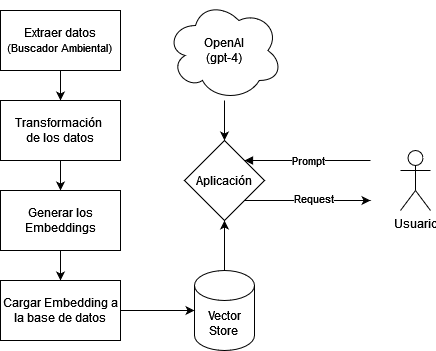
\includegraphics[width=.5\textwidth]{figures/huemul1.png}
    \caption[Estructura basica de la aplicación]{Estructura basica de la aplicación\\
    {\scriptsize (Fuente: Elaboración propia)}}
    \label{fig:logoind}
\end{figure}
    

A partir de esta estructura mientras se avance en el desarrollo, se explicará parte por parte el proceso y con ello los riesgos de cada uno de ellos.



\section{ETL}


Para realizar el proyecto fue necesario realizar un proceso de ETL. El término ETL se refiere a las técnicas de "Extracción, 
Transformación y Carga" (Extract, Transform, Load), que constituyen un proceso clave para los datos necesarios para el proyecto. 
Este proceso implica la extracción de datos de fuentes heterogéneas, su transformación para ajustarse a las necesidades del 
negocio y su posterior carga en un destino que, por lo general, es un almacén de datos diseñado para el análisis y la generación 
de informes\cite{ETL1}.

% Inclusión de Figuras
\begin{figure}[ht!]
    \centering
    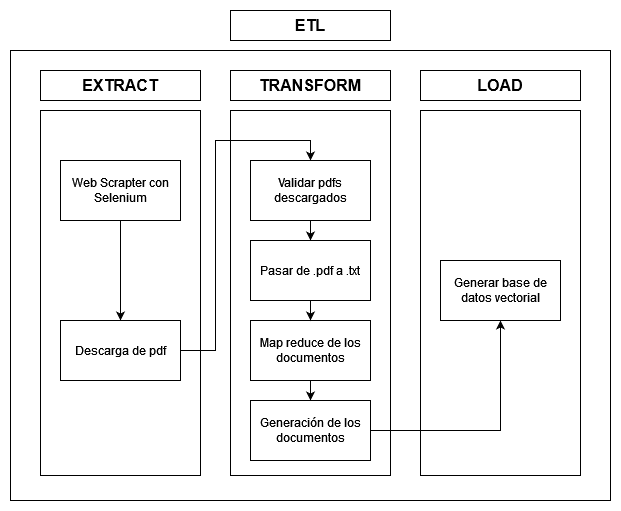
\includegraphics[width=.5\textwidth]{figures/huemulETL.png}
    \caption[Estructura del proceso de ETL para el Buscador Ambiental]{Estructura del proceso de ETL para el Buscador Ambiental\\
    {\scriptsize (Fuente: Elaboración propia)}}
    \label{fig:etl1}
\end{figure}
    

La fase de extracción implica la recolección de datos de múltiples fuentes, que pueden variar desde bases de datos 
estructuradas hasta información no estructurada en la web. La transformación se refiere al proceso de limpieza, conversión, 
y consolidación de estos datos en un formato adecuado para el análisis. Finalmente, la carga es el proceso de transferir 
los datos transformados al sistema de destino, donde se pueden almacenar y utilizar para la toma de decisiones estratégicas 
\cite{ETL1}.

\subsection{Extract}

%\autoref{fig:logoind}

La información requerida para el desarrollo del Chatbot se obtuvo del "Buscador ambiental" del Tribunal de Protección Ambiental 
de Chile a través de su sitio web\cite{BuscadorAmbiental}. Este portal aloja todos los documentos públicos disponibles para su consulta en cualquiera 
de los tres tribunales ambientales. Para acceder a la base de datos necesaria, se llevó a cabo la creación de 
un bot capaz de recopilar las entradas de este buscador de manera análoga a un usuario convencional.

\begin{figure}[ht!]
    \centering
    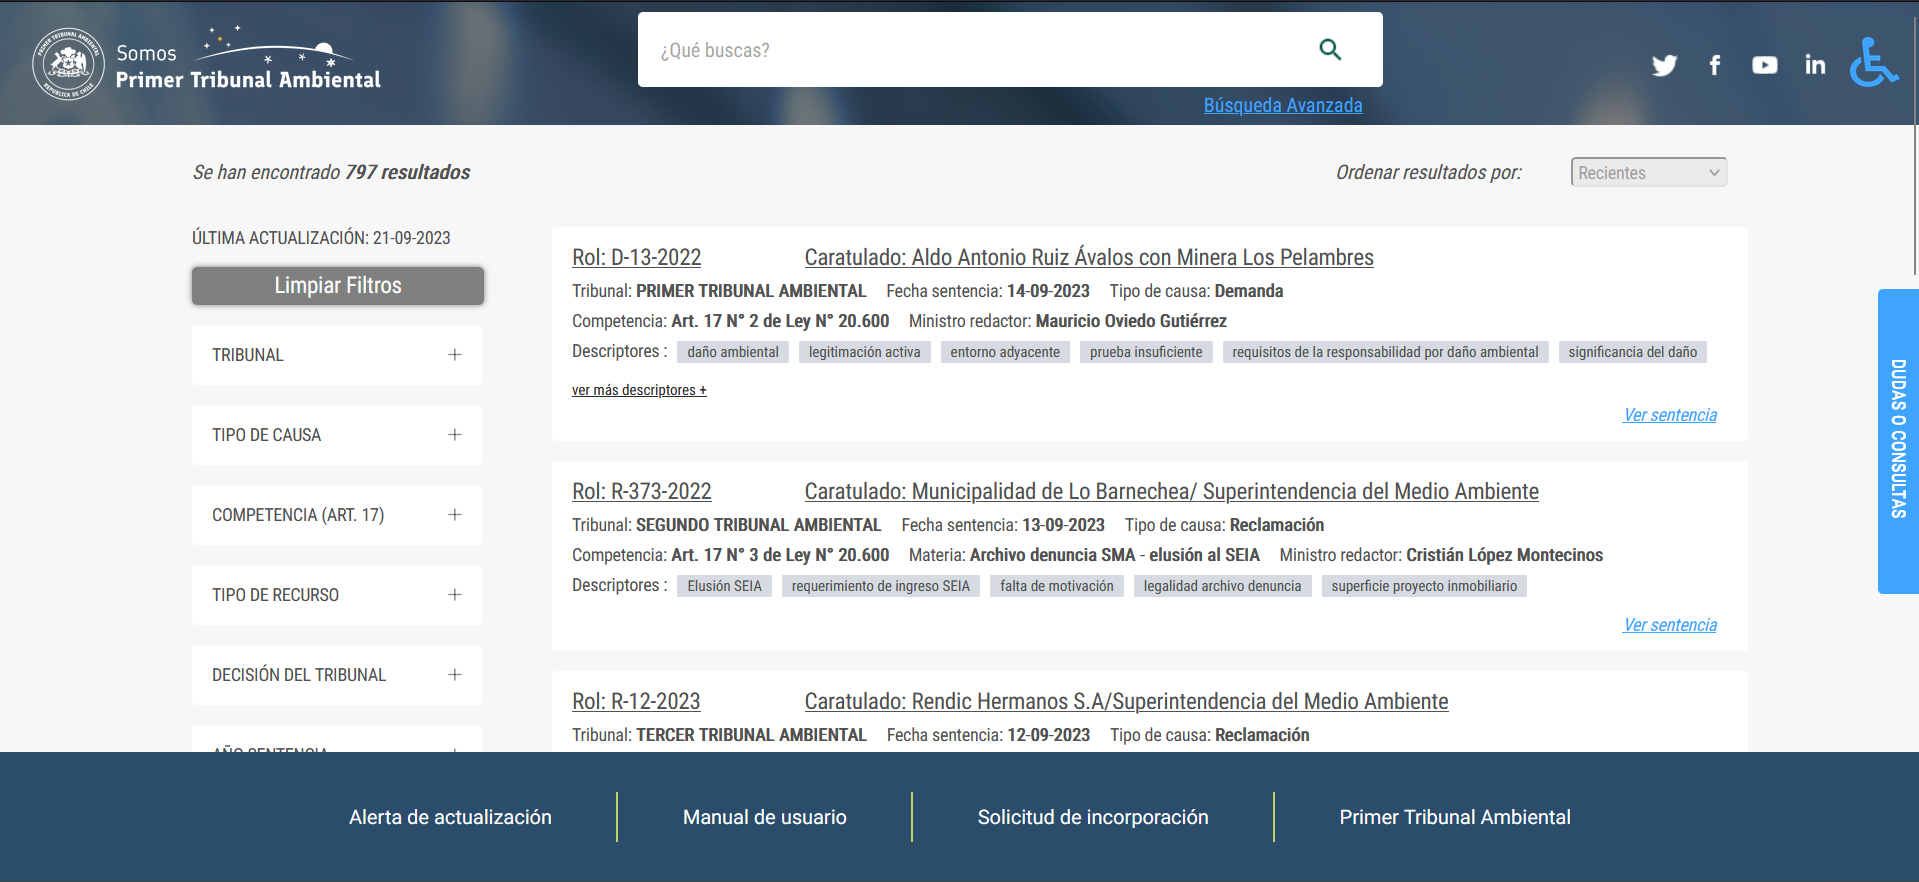
\includegraphics[width=.8\textwidth]{figures/huemul2.png}
    \caption[Screenshot del Buscador de la pagina del Primer Tribunal Ambiental]{Buscador de la pagina del Primer Tribunal Ambiental\\
    {\scriptsize (Fuente: Pagina del Primer Tribunal Ambiental)}}
    \label{fig:extract1}
\end{figure}
    
Para esta tarea, se empleó Selenium, una herramienta originalmente diseñada para generar pruebas, pero que, debido a la naturaleza 
reactiva y dinámica de los sitios web, así como a la detección de bots por parte de algunas páginas, resultó ser la elección 
más apropiada. Este bot, después de explorar todas las páginas del buscador ambiental, como se ilustra en la \autoref{fig:extract1},
logró recuperar cada uno de los enlaces individuales que conducen a las páginas específicas de cada caso, tal como se 
muestra en la \autoref{fig:extract2}.

\begin{figure}[ht!]
    \centering
    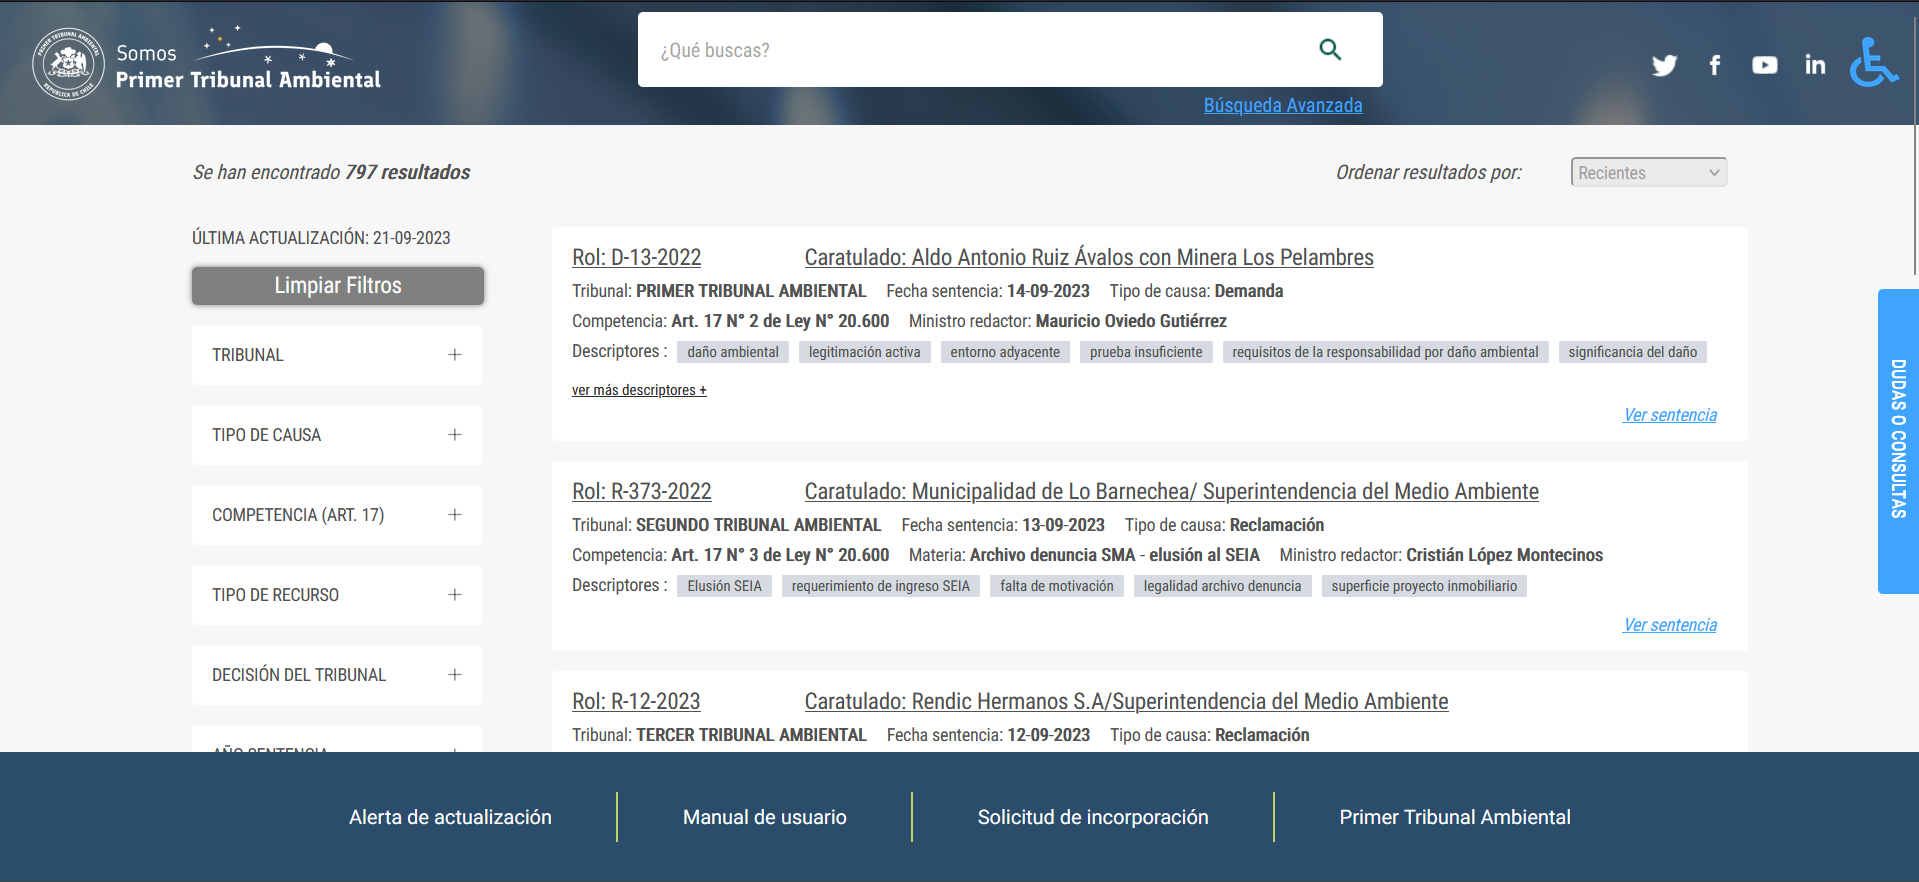
\includegraphics[width=.8\textwidth]{figures/huemul2.png}
    \caption[Screenshot de una sola reclamación en la pagina web del buscador ambiental]{Screenshot de una sola reclamación en la pagina web del buscador ambiental\\
    {\scriptsize (Fuente: Pagina del Primer Tribunal Ambiental)}}
    \label{fig:extract2}
\end{figure}
    
Posteriormente, se contemplaba la posibilidad de obtener tanto los enlaces a cada documento en formato PDF como la información 
detallada de cada uno de estos documentos mediante la creación de un nuevo bot. Sin embargo, durante el proceso de desarrollo 
de este bot, se logró acceder a la API que permitía obtener directamente todos los datos mencionados anteriormente. Esto suprimió 
la necesidad de crear otro tipo de bot utilizando Selenium, ya que bastaba con realizar una solicitud a la mencionada API.

Para completar la fase de extracción de datos (Extract), una vez que se había obtenido toda la información mediante las solicitudes 
a la API, el último paso consistió en generar nuevas solicitudes con el objetivo de descargar todos los archivos PDF de cada una 
de las entradas. Estos archivos ahora están descargados y listos para la próxima etapa del proyecto, que implica la transformación 
de los datos con el fin de obtener la información necesaria para construir la base de datos a partir de los documentos.


\subsection{Transform}

\par En la continuación del proceso de ETL (Extracción, Transformación y Carga), los PDFs que previamente han sido descargados 
requieren ser sometidos a modificaciones con el objetivo de convertir la información que inicialmente se presenta en un 
estado "sucio" en datos "limpios" que puedan ser adecuadamente utilizados en el proyecto. Este proceso se denomina 
"transformación," o "transform," en inglés.

\par Entre los datos descargados, nos encontramos con un extenso número de PDFs que presentan dificultades significativas para su 
manipulación. Esto se debe a que el Tribunal Ambiental no sigue un formato estándar en la estructura de las reclamaciones 
presentadas. En consecuencia, cada uno de los textos posee un formato propio, lo que complica en gran medida la extracción 
eficiente de las diversas secciones contenidas en dichos textos. Sin embargo, gracias al funcionamiento del proceso de semejanza 
semántica, esta diversidad de formatos no representa un problema insuperable para el proyecto.

\par No obstante, surgen dificultades adicionales cuando se trata de las reclamaciones que son presentadas a los tribunales ambientales 
en formato digital o, en su defecto, en forma de fotocopias. Esto implica que no todos los documentos están habilitados para su 
procesamiento. En consecuencia, el primer paso en el proceso de transformación involucra la discriminación de qué PDFs son 
susceptibles de ser procesados y cuáles no. Para llevar a cabo esta tarea, se ha desarrollado un script capaz de detectar 
texto dentro de un archivo PDF. Si el texto es legible, se almacena; de lo contrario, se elimina.

\par Una vez separados los PDFs legibles y adecuados para el trabajo posterior, se procede con la transformación de estos documentos 
al formato TXT (texto plano). Esta etapa se lleva a cabo considerando la conveniencia de trabajar con archivos en formato de 
texto en comparación con los archivos en formato PDF puro, dado que el próximo método de transformación, que implica el uso de
 map-reduce en Langchain, requiere que los datos estén en formato de texto.

 \par Dentro del contexto del uso de Langchain, el proceso de map-reduce implica, en primer lugar, la aplicación de una cadena de 
LLM (Modelo de Lenguaje de Gran Tamaño) a cada documento individual {docs[i]}, considerándolos de manera independiente 
(la fase de "Map"). Esto implica tratar la salida de la cadena como un nuevo documento, resumido. Posteriormente, todos los 
nuevos documentos resumidos se envían a una cadena de combinación de documentos para obtener una única salida por archivo 
(la fase de "Reduce"). En este contexto, la implementación de map-reduce en los archivos de texto (TXT) conlleva la aplicación 
de la cadena de LLM a cada documento de manera individual, generando así una nueva representación del mismo.

\par Sin embargo, es importante destacar que un archivo .txt puede contener un número de tokens demasiado elevado como para ser 
reducido de manera inmediata. En situaciones de este tipo, es necesario recurrir a un proceso de subdivisión que fragmente los 
textos en segmentos con un número de tokens inferior al límite impuesto por la API de OpenAI. Cada archivo .txt puede ser dividido, 
resumido y exportado a un nuevo archivo .txt una vez que ha sido fragmentado previamente en segmentos.

\par Los documentos procesados son combinados utilizando otra cadena de procesamiento para obtener un resultado final consolidado. 
Para concluir el proceso de transformación, los resúmenes generados después de haber pasado por el procedimiento de map-reduce 
se someten a un último paso antes de ser incorporados en la base de datos. Este paso implica la fusión de los resúmenes con la 
información obtenida a través de las solicitudes a la API del Tribunal Ambiental, presentada en formato de texto. Este proceso 
resulta en la creación de un único documento que engloba toda la información, al cual nos referiremos como "documentos finales". 
Con esto, se concluye la fase de transformación y se procede al último procedimiento, conocido como "carga" (Load), que consiste 
en cargar estos documentos finales en la base de datos.


\subsection{Load}

\par Al culminar el proceso de Extracción, Transformación y Carga (ETL), resulta fundamental llevar a cabo la fase de carga, 
también conocida como "load" en inglés, en la cual se incorporan todos los descriptores previamente descargados y transformados 
en una base de datos. Para este proyecto, en el cual se utiliza LangChain, resulta de vital importancia fragmentar los documentos 
en secciones más pequeñas.

\par Esta necesidad surge debido a que los documentos deben ser sometidos a un proceso de incrustación (embedding) antes de ser 
introducidos en la base de datos. Esto se debe principalmente a que las funciones de incrustación tienen un límite en la extensión 
de grupos de caracteres, conocidos como "tokens," que pueden ser procesados. En el contexto del modelo de incrustación 
"text-embedding-ada-002," este límite se establece en 8191 tokens [1], lo que constituye la longitud máxima de los fragmentos.

\par Por lo tanto, cuando se trabaja con documentos extensos, es imperativo dividirlos en fragmentos más pequeños antes de proceder 
con su incorporación. Según la información proporcionada en el Blog de OpenAI, los embeddings son "representaciones numéricas 
de conceptos convertidos en secuencias numéricas, lo que facilita que las computadoras comprendan las relaciones entre los 
conceptos." En términos sencillos, los embeddings son representaciones vectoriales de texto que permiten su comprensión por 
parte del Modelo de Lenguaje de Gran Tamaño (LLM). Dado que los LLM son redes neuronales, el proceso de incrustación resulta 
esencial para traducir el texto en números, que es el formato comprensible para esta red neuronal basada en Transformers.

\par Los embeddings resultantes se almacenan posteriormente en una base de datos vectorial denominada ChromaDB. Esta base de 
datos ha sido diseñada para ser compacta, escalable y eficiente, con el propósito de almacenar y recuperar vectores de manera 
efectiva. ChromaDB genera índices que permiten una recuperación rápida y eficiente de los embeddings en función de las 
consultas realizadas por los usuarios.

\section{Chatbot}



\chapter{Resultados}

Esta tesis, al presentar una solución a un problema basado en el lenguaje natural (NLP), enfrenta el desafío de cuantificar 
los resultados entregados por el chatbot en respuesta a nuestras consultas. Debido a esta complicación, se propone utilizar 
una escala para evaluar dichos resultados en los ejemplos de la siguiente manera:

\begin{enumerate}
    \item \textbf{Satisfactorio}: La respuesta es acorde a lo que menciona el prompt.
    \item \textbf{Medianamente Satisfactoria}: La respuesta es adecuada, pero incluye errores que, si bien no invalidan la respuesta, podrían generar confusión.
    \item \textbf{Insatisfactorio}: La respuesta no es pertinente o incluye información inventada.
\end{enumerate}

Dada esta metodología para evaluar los casos, se presentarán ejemplos de prompts que un usuario podría emplear habitualmente 
en el uso de la aplicación. Se analizarán tanto el contexto enviado por el chatbot a OpenAI, como son resultados obtenidos y se 
realizara un contraste con la información de la que ya disponemos del periodo de desarrollo.

\section{Caso 1: Consultar por resumen}


\begin{table}[ht!]
    \centering
    \caption[Ejemplo: Primer Prompt]{Primer ejemplo de resultado usando un prompt}
    \begin{tabular}{p{3cm}p{12cm}}
        \toprule
        \textbf{Prompt} & \textbf{Respuesta} \\
        \hline\hline
        Dame un resumen del caso Dominga & El caso Dominga se refiere a una reclamación presentada por Andes Iron SpA contra la Resolución Exenta N° 1146/2017 del Servicio de Evaluación Ambiental y el Comité de Ministros. El reclamo se basa en el rechazo del Estudio de Impacto Ambiental del proyecto Dominga y la acogida parcial de los recursos de reclamación presentados en el marco de la participación ciudadana. El Primer Tribunal Ambiental de la República de Chile admitió la reclamación y convocó a una audiencia de percepción documental. Además, se presentaron informes de Amicus Curiae y se aceptó la participación de terceros coadyuvantes e independientes. El proceso judicial continúa y se espera una sentencia definitiva. En una sentencia anterior, el tribunal rechazó la excepción de extemporaneidad interpuesta por un tercero independiente y acogió la reclamación presentada por Andes Iron SpA. Sin embargo, la Corte Suprema anuló la sentencia y remitió el caso nuevamente al Primer Tribunal Ambiental para que se pronuncie sobre el fondo del asunto. El caso involucra diversos hechos controvertidos, como la evaluación del proyecto, la suficiencia de la información, los impactos ambientales, las medidas de compensación y la participación ciudadana.  \\
        \bottomrule
    \end{tabular}
    \label{tb1:prompt1}
\end{table}

Una de las consultas más evidentes podría ser la solicitud de un resumen de alguna de las reclamaciones mandadas al Tribual; por lo tanto, 
es esencial evaluar el desempeño de este proceso con dicho prompt.

Como se puede observar en la respuesta proporcionada por el Chatbot, esta parece ser aceptable y lógica. Sin embargo, es necesario comprender 
ciertos aspectos. En primer lugar, enviar el prompt con el nombre del proyecto en lugar del código mejora la calidad de búsqueda, ya que los 
vectores de embedding reconocen más eficientemente las diferencias semánticas, proporcionando un contexto más adecuado. Además, es importante 
considerar que el envío de un exceso de contexto puede generar ``alucinaciones'', resultando en resúmenes que no sean completamente precisos o que 
contengan información falsa generada por el LLM. El contexto enviado a OpenAI por el chatbot en el ejemplo y que contiene más contexto del necesario
 se encuentra en el \autoref{appx:contexto}. A pesar de los puntos anteriores, podemos decir que la respuesta entregada por el chatbot es \textbf{Satisfactoria}.

\section{Caso 2: Consulta por listado}

\begin{table}[ht!]
    \centering
    \caption[Ejemplo: Segundo Prompt]{Segundo ejemplo de un punteo o listado con todas la reclamaciones relacionadas con Humedales}
    \begin{tabular}{p{3cm}p{12cm}}
        \toprule
        \textbf{Prompt} & \textbf{Respuesta} \\
        \hline\hline
        Dame un punteo o listado con todas la reclamaciones relacionadas con Humedales& A continuación se presenta un listado con todas las reclamaciones relacionadas con Humedales: 1. Caso Humedal La Marina: - Rol: ``R-25-2021'' - Fecha: 31-03-2022 - Reclamante: Inversiones F.K Limitada - Materia: Declaración humedal urbano - Resolución: Rechazada por el Third Environmental Court 2. Caso Humedal Urbano "Estero Agua Salada": - Rol: ``R-354-2022'' - Fecha: 19-07-2023 - Reclamante: Consorcio Punta Puyai S.A. - Materia: Declaración humedal urbano - Resolución: Rechazada por el Second Environmental Court 3. Caso Humedal Quilicura: - Rol: ``R-297-2021'' - Fecha: 24-10-2022 - Reclamante: Inversiones Butamalal S.A. y otros - Materia: Declaración humedal urbano - Resolución: Acogida parcialmente por el Second Environmental Court 4. Caso Humedal El Bosque-Miraflores-Las Multas-Guacamayo: - Rol: ``R-37-2021'' - Fecha: 10-03-2023 - Reclamante: Nicolás Reichert Haverbeck - Materia: Declaración humedal urbano - Resolución: Acogida por el Third Environmental Court Espero que esta información sea de utilidad.  \\
        \bottomrule
    \end{tabular}
    \label{tb1:prompt1}
\end{table}

Otra consulta común es preguntar por listados a partir de la información del tribunal ambiental, este tiempo de preguntas resulta tener una dificultad engañosa para el Chatbot.
Tras analizar la respuesta, se identifican aspectos tanto positivos como negativos. Entre los positivos, destaca que el Modelo de Lenguaje de Gran Escala (LLM) 
comprende correctamente el concepto de listado, generando una lista de cuatro resultados pertinentes. No obstante, se observa una limitación significativa: 
la base de datos vectorial incluye más de 20 documentos relacionados con humedales, pero debido a la restricción de enviar únicamente entre 3 a 5 
documentos como contexto por parte del chatbot, no todos estos documentos pueden ser procesados para generar una respuesta correcta. Esta limitación 
resulta en una respuesta que, si bien es veraz, no es completa. Por lo tanto, aunque la información sobre humedales es incompleta, la respuesta puede 
calificarse como \textbf{Medianamente Satisfactoria}, basándose en la precisión de los datos proporcionados y la capacidad del sistema para entender y 
organizar la información relevante en un formato de listado.

\newpage

\section{Caso 3: Comparación entre reclamaciones}

\begin{table}[ht!]
    \centering
    \caption[Ejemplo: Tercero Prompt]{Tercer ejemplo comparación entre reclamaciones}
    \begin{tabular}{p{3cm}p{12cm}}
        \toprule
        \textbf{Prompt} & \textbf{Respuesta} \\
        \hline\hline
        Compara la reclamación R-25-2021 con la reclamación R-1-2017& La reclamación R-25-2021 se refiere al caso del Humedal La Marina, mientras que la reclamación R-1-2017 se refiere al caso de Dominga. Ambas reclamaciones son presentadas por diferentes partes en contra del Ministerio del Medio Ambiente y se centran en la evaluación ambiental de los respectivos proyectos. En el caso del Humedal La Marina, la reclamante argumenta que la solicitud de reconocimiento del humedal no cuenta con el acuerdo del Concejo Municipal y que se violó el debido proceso por falta de emplazamiento. Además, cuestiona la forma de notificación de los actos administrativos y la falta de motivación en la resolución reclamada. También acusa que la resolución incurre en desviación de poder y solicita que se deje sin efecto. Por otro lado, en el caso de Dominga, la reclamación se basa en el rechazo del Estudio de Impacto Ambiental del proyecto minero-portuario. Los reclamantes argumentan que se aplicaron incorrectamente los criterios de evaluación y que se omitieron estudios relevantes. También cuestionan la forma de notificación de los actos administrativos y la falta de motivación en la resolución reclamada. En este caso, la reclamante solicita que se modifique la resolución para no afectar su derecho de propiedad. En resumen, ambas reclamaciones se centran en la evaluación ambiental de los proyectos y cuestionan aspectos como la falta de acuerdo del Concejo Municipal, la forma de notificación de los actos administrativos, la falta de motivación en las resoluciones y la posible desviación de poder. Sin embargo, cada reclamación se basa en circunstancias y argumentos específicos relacionados con los proyectos y los humedales involucrados.\\
        \bottomrule
    \end{tabular}
    \label{tb1:prompt1}
\end{table}

La propuesta de utilizar un prompt que busca comparar la relación entre dos textos representa una aplicación práctica y avanzada de un Modelo de 
Lenguaje de Gran Escala (LLM), más allá de su función como simple buscador. Esta metodología permite al LLM demostrar su habilidad para no solo 
identificar, sino también para analizar y comparar de manera fluida y sencilla los contenidos de diferentes documentos. En el ejemplo proporcionado, 
el LLM logra distinguir y describir cada texto antes de proceder a una comparación efectiva.

Sin embargo, se presenta una limitación similar a la observada en el primer ejemplo. Al revisar los contextos enviados a OpenAI revela que documentos
no relacionados fueron incluidos en dicho contexto, lo cual, aunque no generó información incorrecta en este caso, tiene el potencial de causar 
alucinaciones. A pesar de este inconveniente, la capacidad del LLM para manejar adecuadamente los documentos relevantes y su eficacia en la 
comparación de textos justifican calificar la respuesta como \textbf{Satisfactoria}.

\newpage

\section{Caso 4: Consultar por información falsa}


\begin{table}[ht!]
    \centering
    \caption[Ejemplo: Cuarto Prompt]{Cuarto ejemplo preguntando por un texto que no existia}
    \begin{tabular}{p{3cm}p{12cm}}
        \toprule
        \textbf{Prompt} & \textbf{Respuesta} \\
        \hline\hline
        Dame un resumen de R-14-2023 & El resumen de R-14-2023 es el siguiente: La Resolución R-14-2023 se refiere al proyecto denominado Centro de Cultivo de Salmónidos ``Córdova 4''. Esta resolución establece las regulaciones y requisitos para la operación y funcionamiento de dicho centro de cultivo. Entre las principales disposiciones de la resolución se encuentran: 1. Autorización para la construcción y operación del Centro de Cultivo de Salmónidos "Córdova 4" en la ubicación especificada. 2. Establecimiento de medidas de protección ambiental para garantizar la preservación de los recursos naturales y la biodiversidad en el área de influencia del centro de cultivo. 3. Requisitos técnicos y de seguridad que deben cumplir las instalaciones del centro de cultivo, incluyendo sistemas de tratamiento de aguas residuales, control de calidad del agua y medidas de prevención de escapes de peces. 4. Obligaciones y responsabilidades del titular del proyecto en cuanto a la gestión adecuada de los desechos generados por el centro de cultivo y la implementación de programas de monitoreo y seguimiento ambiental. 5. Procedimientos y plazos para la presentación de informes periódicos sobre el estado y desempeño del centro de cultivo, así como para la realización de inspecciones y auditorías por parte de las autoridades competentes. Es importante destacar que este resumen es una síntesis de la resolución y no reemplaza la lectura y comprensión completa del documento original. Se recomienda consultar la resolución R-14-2023 en su totalidad para obtener información detallada sobre todas las disposiciones y requisitos establecidos.\\
        \bottomrule
    \end{tabular}
    \label{tb1:prompt1}
\end{table}

Con el objetivo de ilustrar un aspecto crucial, se realizó una consulta al LLM utilizando información inexistente, específicamente la reclamación R-14-2023 
que se inventó. Como era de esperarse, al solicitar información sobre un tema falso, el LLM generó una respuesta igualmente falsa. Este fenómeno se debe a 
que el chatbot ejecuta un proceso de semejanza semántica entre el prompt y los documentos disponibles, mandando estos documentos como contexto a OpenAI, 
esto pasa porque el chatbot no tiene como discernir si es necesario el proceso o no.

Este experimento subraya una limitación significativa del LLM: su incapacidad para discernir la veracidad de los datos en la consulta inicial. 
Dado que el modelo se basa en la información proporcionada, cualquier inexactitud en el prompt puede llevar a respuestas erróneas. 
Esta característica del LLM plantea preocupaciones particulares en contextos donde la fiabilidad y precisión de la información son fundamentales. 
En consecuencia, se considera que la respuesta obtenida en este caso es completamente insatisfactoria.





\chapter{Evaluación de Riesgos}

En el dinámico campo de la Inteligencia Artificial, particularmente en el ámbito de los Modelos de Grande de Lenguaje (LLM), 
la evaluación de riesgos es un elemento crucial para el éxito y la viabilidad de cualquier proyecto. Este sección se dedica 
a explorar los desafíos y consideraciones esenciales en el desarrollo y aplicación de proyectos basados en LLM, ofreciendo 
una perspectiva integral sobre cómo mitigar riesgos y optimizar el rendimiento de estos modelos.

Al abordar la Evaluación de Riesgos en proyectos que involucran LLM, es indispensable considerar varios factores críticos 
que pueden influir directamente en el resultado del proyecto. Estos factores pueden aparecer tanto en el periodo de creación
del proyecto, como mientras aplicamos la tecnología. A continuacion, se presetaran una serie de riegos que hay que tener en 
consideracion para cualquier proyecto que utilice como base los LLM.

\section{Creación del Proyecto}

\subsection{No tener un análisis previo de que se busca lograr}

La realización de un análisis previo, tanto de una aplicación como un proyecto, resulta crucial para el inicio de cualquier 
proyecto basado en datos, independiente de la rama en donde se esté aplicando, donde el NLP no es la excepción. 
La mayoría de los usuarios que tienen acceso a herramientas analíticas, realmente no entienden el funcionamiento interno de dichas herramientas \cite{datos1}, 
por consiguiente, es crucial que al empezar un proyecto se entienda a la perfección donde se quiere llegar, realmente necesita y cuáles son los objetivos. 

Además, es común que suceda, que en un conjunto de datos muy extenso, cualquier efecto que desee probar aparecerá como significativo \cite{datos1}, de ahí la 
importancia de un análisis previo de objetivos y problemáticas. Este proceso es tan importante, debido a que existen casos en donde un problema que puede resultar complejo en 
primera instancia, puede sugerir el uso de modelos muy complejo. Sin embargo, usando un modelo más simple se llegan a resultados mejores 
que con el uso de complejo \cite{datos2}, siendo este tipo de escenarios, un ejemplo claro de que un análisis previo adecuado puede mejorar tanto los resultados como la 
experiencia de desarrollo al trabajar. 

\newpage

\subsection{Calidad de los datos}

Para cualquier tipo de trabajo, aplicación o estudio, la calidad de los datos es en extremo importante esto debido a que, la calidad de los datos 
es crítica para un sistema de Machine Learning, porque los datos deficientes podrían causar problemas graves como predicciones erróneas o baja 
precisión de clasificación \cite{calidad1}. Ahora si hablamos del uso de LLM, que forma parte del procesamiento del lenguaje natural, además del Deep learning, 
simplificamos los atributos de calidad de datos en los tres más importantes para el Deep Learning: la fidelidad, la variedad y la veracidad de un conjunto de datos \cite{calidad1}.

Como ejemplo, un caso que sucedió dentro del proyecto que acompaña a este análisis de riesgo, se tuvo problemas en una ciertas cantidad reclamaciones tratadas en el proceso 
de ETL, esto debido principalmente a que el Tribunal ambiental no cuenta con un estándar para entregar las reclamaciones que luego aparecerán en el buscador ambiental, existían tanto pdf que eran legibles, como otros 
que eran solo fotocopias, lo que imposibilitaba la extracción de información por problemas de formatos. El problema la calidad de los datos a su vez, se puede extrapolar a la 
calidad de la metadata que era anexa en la base de datos dentro del proyecto.

\subsection{Sesgos} %sesgo2

Los Modelos de Lenguaje Grande (LLM), al ser entrenados con una masiva cantidad de datos, pueden manifestar sesgos debido al origen y procedencia de los datos utilizados en su entrenamiento. Estos sesgos pueden dar lugar a desafíos en desarrollos cuando se aplican en 
contextos distintos, ya que las respuestas generadas por el modelo pueden no ser adecuadas ni ajustarse a la realidad de 
esos nuevos escenarios, llevando así a respuesta erróneas, inexactas e incluso a respuestas discriminadoras.

Dentro de los muchos problemas que estos sesgos pueden generar algunos ejemplos son: 
Estereotipos de género en elección de ocupaciones, inexactitud ante las ambigüedades de una frase, dificultad de entender dinámicas complejas de género, sesgos culturales, discrepancia en las explicaciones de los modelos, etc. \cite{bias1}
Esto sucede porque los modelos preentrenados con corupus generados por humanos contienen sesgos sociales hacia ciertos grupos demográficos, porque el humano es un ser lleno de sesgos y con ello también los textos que produce. Estos sesgos son preocupantes, debido a que pueden ser propagados o incluso amplificados en las tareas que estos modelos realizan \cite{sesgo2}, pudiendo llegar a malas repuestas o en el peor de los casos problemas legales.

Como ejemplo podemos citar el dicho por Bill Gates en su entrevista ``Can AI Save the World? Expert Insights with Bill Gates'' en donde menciono que: 
``Los sesgos en los modelos de IA pueden llevar a diagnósticos incorrectos, como se vio en el ejemplo donde Chat GPT diagnosticó erróneamente la 
tuberculosis como gripe debido a las bajas tasas de tuberculosis en los EE. UU.'' \cite{billgates1}. Con este ejemplo, es que podemos dimensionar el efecto real de estos sesgos y
en lo correcto o incorrecto que puede llegar a ser una respuesta por parte de estos modelos.

\subsection{Elección correcta del modelo}
Actualmente la oferta de grandes modelos de lenguaje tanto para investigación (research) como desarrollo comercial es muy amplia, podemos encontrar desde los privados como: ChatGPT, PaLM, Bloom, etc. 
Como también modelos de código abierto y libres para su uso comercial como: Llama 2, OpenLLaMA, Falcon, Dolly, etc. \cite{modelos2} Cada uno con sus respectivas variantes, debido a que existen 
variantes del modelo siendo unos más potentes que otros, a pesar de ser de la misma familia. Como por ejemplo tenemos a Llama 2 que se puede encontrar en versión de 7, 13 y 70 billones de parámetros \cite{modelos3}. 

La elección de un modelo correcto para trabajar es sumamente importante parar el desarrollo, esto debido a que tanto la diversidad y calidad de los datos de preentrenamiento influyen 
sustancialmente en la capacidad del modelo de lenguaje para comprender y proporcionar respuestas precisas, el tamaño puede tener una 
gran influencia en el rendimiento, además cada modelo tiene su el soporte lingüístico \cite{modelos1}, lo que dependiendo del tipo de proyecto podría ser crucial y determinante para el éxito de este.  


\subsection{Costos Monetarios}
Los costos relacionados con la puesta en producción, en caso de usar un modelo open source, o el uso de un modelo LLM, considerando el uso de un LLM privado, pueden aumentar de manera exponencial si es que no se planea con antelación el costo monetario de ellos o no se predice la demanda de manera adecuada. Por lo tanto, es fundamental tener en 
cuenta los costos asociados al utilizar un servicio de tercero, así como el costo de operar un servidor local, que pueden incluir el consumo de energía eléctrica, como la compra de tarjetas gráficas (GPU) para el funcionamiento correcto y optimo de los modelos.
Por ejemplo, existen estudios en donde al realizar ajustes al modelo, también llamado fine tunning, es consumo de energía es comparable al de pequeñas ciudades y el dióxido 
de carbono emitido es equivalente a 500 veces la de un vuelo de ida y vuelta entre Nueva York y San Francisco \cite{ft1}, por lo cual es un factor que hay que tener en cuenta. 


\subsection{Funciones de Embedding}

Como se mencionó anteriormente en esta tesis, las funciones de Embedding son específicas para cada gran modelo de lenguaje y no son intercambiables entre modelos. Esto se debe a que los embeddings son 
representaciones de alto nivel provenientes de los pesos y parámetros de cada modelo, por lo que están diseñadas para captar y almacenar las relaciones semánticas específicas de cada modelo \cite{microsoft1}. Por lo que, si se desea usar un modelo grande de lenguaje, es necesario contar con su función de Embedding correspondiente, además de la capacidad computacional para hacer funcionar dicha función, porque de lo contrario el modelo no podrá obtener el vector necesario de entrada para generar la predicción y con ello no podrá generar una respuesta. 


\subsection{Conocimiento de Framework}
Cuando se desarrolla una aplicación, es esencial comprender el funcionamiento interno de los frameworks o herramientas que se utilizaran a lo largo del proyecto. 
Esta comprensión no solo es valiosa para entender el cómo funciona proceso en su conjunto, sino que también es necesaria para tener un control los costos asociados al 
proyecto en caso de llevarse a producción.  

Por ejemplo, en el contexto del proyecto de esta tesis, es importante saber que el framework Langchain, suele realizar múltiples llamadas a los modelos \cite{framework1}. Si no se tiene conocimiento de esta situación o no se cuantifican de manera adecuada 
la cantidad de llamadas y la extensión de estas, esto debido a que los modelos como los entregados por OpenAI tiene un costo por lo tokens que se reciben y por los que se envían \cite{openaimodels}, esto puede dar lugar a problemas en la cuantificación de costos. Por lo tanto, la capacidad de comprender y 
medir con precisión el uso de recursos, como las llamadas a los modelos, es esencial para gestionar eficazmente los costos y asegurar el éxito del proyecto para cuando este sea enviado a producción.


\subsection{Volatilidad del Mercado}

Considerando a la fecha actual en donde se está escribiendo esta sección de la tesis, el 06 de noviembre de 2023, la creación de Chatbots utilizando la metodología RAG se perfilaba como 
una de las tendencias más destacadas en el mercado, siendo posiblemente una de las aplicaciones más prometedoras que los LLM tendría hasta la fecha. 
No obstante, en este mismo día, se llevó a cabo la OpenAI DevDay Keynote, donde se anunciaron novedades significativas en la oferta de productos por parte de la empresa OpenAI, como por ejemplo la entrada en 
escena de los GPTs, que permite personalizar versiones de ChatGPT con instrucciones, conocimiento extra y cualquier otra combinación 
de habilidades \cite{openai2}. Junto con ello a su vez, se introdujeron nuevos modelos al catálogo de su API como gpt-4-turbo, un playground de desarrollo más completo para el desarrollo con herramientas de la empresa, 
text-to-speech (TTS), entre otros \cite{openai3}.

Con este contexto, es comprensible que comprometerse con cualquier tecnología conlleva riesgos, especialmente en este período caracterizado por una 
volatilidad extrema y una inversión extremadamente agresiva en inteligencia artificial. La Inteligencia Artificial Generativa 
continúa evolucionando de manera acelerada, lo que la hace cada vez más disruptiva y eficiente. Por lo tanto, la investigación 
y la implementación de soluciones de inteligencia artificial centradas en asistentes o chatbots representan un compromiso de alto 
riesgo en este entorno en constante cambio a la espera de nuevos servicios y competidores.


\newpage

\section{Uso de la Aplicación}

\subsection{Alucinaciones}

En un contexto de uso de grandes modelos de lenguaje, el termino ``alucinación'' se refiere a la generación de textos o respuestas que exhiben corrección gramatical, fluidez y autenticidad,
pero se desvían de las entradas de fuente proporcionadas (fidelidad) o no se alinean con la precisión factual (factualidad) \cite{alucionacion1}.
Explicando lo anteriormente dicho en términos más simples, decimos que un LLM alucina cuando las respuestas del modelo son coherentes y cohesiva, pero que sin embargo presenta información errónea o una lógica errada, también de una manera más coloquial podríamos decir que el modelo entrega información inventada a las preguntas que se le hacen.   

Dicho lo anterior, podemos decir que este es un gran factor de riesgo para el uso de una aplicación, sobre todo si de su respuesta depende la toma de decisiones sensibles, porque a pesar de estar usando una 
metodología RAG, que dificulta la posibilidad de generar alucinaciones, sigue estando la posibilidad de que estas sucedan lo que puede 
entregar una respuesta con información errónea o inventada. Si es que las respuestas entregadas por un LLM no se revisa con criterio, se podría a llevar a cometer graves errores al hacer uso de información que es directamente falsa.


\subsection{Entrega de contexto adecuado}

Los LLM a menudo suelen presentan alucinaciones, por lo que es esencial trabajar en reducir la frecuencia de este fenómeno. 
Para lograrlo dicho cometido, la provisión de contexto dentro del prompt para guiar la respuesta no es simplemente un capricho, sino que resulta 
absolutamente indispensable para la exactitud de la respuesta. De hecho, la entrega de contexto adecuado dentro del prompt ha demostrado 
ser una medida altamente efectiva para reducir las alucinaciones, logrando una disminución de hasta un 
99.88 porciento en algunos casos \cite{riego1}.

Por consiguiente, la correcta entrega de contexto dentro del prompt desempeña un papel fundamental en 
la generación de respuestas precisas a las consultas. Esto sucede principalmente porque, ya sea que el contexto 
proporcionado sea correcto, incorrecto o incluso irrelevante, el modelo de lenguaje lo utilizará como base 
para generar sus respuestas.

En el proyecto realizado en esta tesis, la generación de respuestas se basa por completo en la entrega de contexto 
dentro del prompt usando la metodología RAG, lo que a veces puede dar lugar a la transmisión de más información de la necesaria en el prompt 
debido al funcionamiento del framework de Langchain. Esto puede llevar a situaciones en las que el modelo, 
influenciado por la información incorrecta o adicional proporcionada, genere respuestas que no reflejan una respuesta en su totalidad correcta.


\subsection{Limitaciones de la similitud de cosenos}

La similitud del coseno, siendo este el método más usado por modelos RAG para la extracción de contexto en una base de datos vectorial, 
como medida de similitud semántica entre los vectores multidimensionales generados por una función de embeddings, particularmente para palabras de alta frecuencia en tareas de 
procesamiento de lenguaje natural (NLP) como preguntas y respuestas (QA), recuperación de información (IR) y traducción 
automática (MT) presenta limitaciones en su uso, esto principalmente sucede debido a que la frecuencia de las palabras en los 
datos de entrenamiento afecta la geometría representacional de los embeddings contextualizados, siendo las palabras de baja 
frecuencias más concentradas geométricamente \cite{coseno}.

Por lo tanto, este problema se extrapola a que, en el momento de querer recuperar contexto pertinente de la base de datos vectorial, 
cuando se realiza el proceso de semejanza semántica por parte del RAG entre el prompt y los vectores de la base de datos, este pueda recibir 
información no relacionada con el prompt, debido a que los vectores que se solicitan siempre son un número fijo y siempre se extrae esa información eligiendo los valores de similitud más altos, por lo que se puede enviar más como contexto del necesario y puede dar oportunidad a alucinaciones.

\subsection{Uso de información privada}

Actualmente las empresas que entregan servicios de LLM son muy herméticos con la manera en que entrenan sus modelos, por lo tanto, no sabemos no sabemos en un 100 por ciento
con qué información han sido entrenados, la cual podría no necesariamente ser solamente información pública. Además, como ejemplo, todas las consultas relizadas en ChatGPT van directamente a los servidores de OpenAI y servirán posteriormente para reentrenar a los modelos de la compañia para mejorar su calidad y performance.

Este tema es ha vuelto tan delicado, que se ha probado que los ataques de reconstrucción de datos son posibles, en ellos se ha propuesto un ataque de reconstrucción dirigido de caja negra donde el 
adversario conoce parte de un ejemplo de entrenamiento (es decir, un indicio de texto) e infiere el resto (por ejemplo, un número de tarjeta de crédito), 
con lo que la posibilidad de extraer datos de entrenamiento de los modelos, lo que representa un riesgo serio para la privacidad \cite{privacidad1}. 

Ante la duda de con que información los modelos son entrenados, actualmente suceden casos como OpenAI que está siendo demandada tanto por violar los derechos de autor \cite{privacidad3} como por robo sistemático \cite{privacidad2} de información, quienes 
demandan alegan que sus obras han sido usadas para entrenar a sus modelos de LLM sin permiso ello y sin pago de regalías. Por lo que, hasta que no tengamos total transparencia del proceso de entrenamiento de estos modelos, 
a pesar de que existen servicios donde la información entregada ``supuestamente'' no es utilizada para reentrenar los modelos de la empresa \cite{openai4}, es preferible ser cautelosos con la 
información que se entrega estos LLM, siempre y cuando estos no estén corriendo de manera local, ya que eso asegura la privacidad de las consultas.



\subsection{Aprendizaje por Refuerzo con Retroalimentación Humana (RLHF)}


Los modelos grandes de lenguaje suelen dar respuestas que a veces, tanto política como moralmente no son correctas, posiblemente debido a la información con sesgos que fue utilizada para su entrenamiento, por lo que 
las empresas tienen por objetivo alinear los valores humanos con los sistemas de aprendizaje automático y dirigir los algoritmos 
de aprendizaje hacia los objetivos e intereses de los humanos \cite{RLHF}. A este proceso se le llama Aprendizaje por Refuerzo con 
Retroalimentación Humana (RLHF). 
Esta intervención de los resultados arrojados por los LLM, puede llegar a ser un problema si mismo, sí se busca realizar una aplicación que tenga por usuario uno con una cultura diferente al proveedor del modelo, este podría generar respuestas no satisfactorias, incluso en caso de que un usuario no pudiera expresase de manera correcta, podría hacer que el modelo se confunda y entregue resultados que podrían ser incompletos o incorrectos.



\chapter{Conclusiones}

\chapter{Conclusiones}

\par Tal como dijo Arthur C. Clarke: ``Cualquier tecnología suficientemente avanzada es indistinguible de la magia''. Nos encontramos 
en un periodo donde la Inteligencia Artificial esta alcanzado capacidades que cada vez nos sorprenden y nos asustan por igual, donde 
posiblemente nos estamos ilusionando al no lograr lo que nos imaginamos en primera instancia, pero nos maravillamos viendo como logra 
cosas que ni siquiera nos imaginamos en un inicio.  

\par El uso comercial de la inteligencia artificial en espacial de lo LLM, como fue la cobertura de esta tesis, presenta una cantidad 
muy alta de riesgos, tanto de los que son fáciles de prevenir como pueden ser los cuantitativos como prevenir costos excesivos en 
servidores como los difíciles de prevenir como las alucinaciones.  Es importante para que estas aplicaciones tengan un buen futuro 
entender tanto como funcionan como de qué manera fueron creadas, los sesgos que presentan estos modelos no dejan de ser un reflejo
de lo que somos y que le dimos de alimento a estos modelos para ser entrenados, siendo un gran reflejo de incluso como somos nosotros 
y la manera en la que actuamos, quedando claro que somos lo que consumimos. 

\par Queda propuesto para quien quiera continuar con esta tesis el entregar resultados más empíricos que pruebas la viabilidad de 
usar en producción este tipo de chatbot, también queda propuesto el solucionar el problema de traer al contexto información que no 
era necesaria propia de la similitud de cosenos. 

\par La industria de la Inteligencia Artificial deja expuesto a absolutamente todos los trabajos desde ahora en adelante en mayor 
o en menor medida, por lo que hay que tener cautela en las decisiones que se toman pues el riesgo es sumamente grande. La 
volatilidad del mercado posiblemente es y será el riesgo más grande por considerar para cualquier tipo de proyecto en el área, 
no fue hace mucho que los llamados Prompt engineer serían los profesionales más cotizados incluso mencionados así por el CEO en 
Nvidia \cite{conclusion1}. Sin embargo, estos fueron ya rápidamente reemplazados por los mismo LLM que se supone tenían que domar, debido a la optimización \cite{conclusion2}
o el auto mejoramiento mediante generación de prompt producidos el mismo LLM, dejando de esa manera obsoleto un rol que hace menos de 
un mes tres meses a la fecha de publicación de esta tesis seria uno de los roles más importantes a futuro.

% Incluir/Eliminar Capítulos
%%!TEX root = ../memoria.tex

\chapter{¿Cómo usar esta Plantilla?}

\section{Obtener el código fuente \LaTeX}

Primero, obtener la plantilla y los archivos de apoyo. Puede hacerlo desde GitHub (\hyperref[https://github.com]{https://github.com}):

\inlinecode{git clone https://github.com/jaimercz/utfsm-thesis}

También existe un formato para presentaciones, basado en \inlinecode{beamer} y en cumplimiento con las disposiciones de la UTFSM para el uso de su imagen corporativa, que puede obtener desde:

\inlinecode{git clone https://github.com/jaimercz/utfsm-beamer}

%%%%%
\section{Configuración}

La configuración básica (nombre del autor, comisión evaluadora, fecha, grado y título de la memoria o tesis) se encuentra en el archivo \inlinecode{config.tex}.

Modifique en este archivo los parámetros básicos de este documento (que afectan la portada y los meta-datos PDF).

\section{Modificación de contenidos}

Abrir el documento maestro (\inlinecode{memoria.tex}) con un editor de texto o editor de \LaTeX{} de su preferencia, y modificar o incluir los documentos que componen su memoria.

Por ejemplo, para incorporar un nuevo capítulo, simplemente puede agregarlo incorporando la siguiente línea en el documento maestro:

\inlinecode{\\input\{includes/capitulo04\}}

\begin{Verbatim}[frame=lines, label=\inlinecode{memoria.tex} (extracto)
				, fontsize=\footnotesize
				, baselinestretch=1
				, formatcom=\color{gray}]
% ... 
% \input{includes/capitulo04}
% \input{includes/capitulo05}
% ... 
\end{Verbatim}

\section{Compilación}

Compilar como todo documento \LaTeX{}.

\begin{Verbatim}[frame=lines, label=Consola (Shell) o Línea de comandos
, fontsize=\footnotesize
, baselinestretch=1
, formatcom=\color{gray}]
    $ pdflatex memoria.tex
    $ biber memoria
    $ pdflatex memoria.tex
    $ pdflatex memoria.tex
\end{Verbatim}

Si hay errores, lo más probable es que le falte alguno de las paquetes necesarios que ocupa esta plantilla\footnote{Más adelante se incluyen los paquetes necesarios; o puedo revirsarlos en \inlinecode{thesis_utfsm.cls} y/o en \inlinecode{thesis_utfsm.sty}.}.

\subsection{Bibliografía}

Esta versión hace uso de \inlinecode{biber} en lugar de \inlinecode{natbib / bibtex}. Natbib es del año 1988, y el manejo de documentos digitales modernos no estaba contemplado entonces.

Puede revisar más sobre \inlinecode{biber} en:
\hyperref[https://ctan.org/pkg/biber]{https://ctan.org/pkg/biber}.

En el archivo maestro puede cambiar/agregar bibligrafía (archivo \inlinecode{bibliography.bib}).

\subsection{Codificación de caracteres}

Todos los archivos \inlinecode{*.tex} de esta plantilla han sido preparados ocupando la codificación de caracteres por defecto \emph{unicode} (UTF-8). Windows (y algunas versiones de OSX) ocupan otro tipo de codificación (ej. \emph{Windows-1252} o \emph{Mac Roman}).

Si deseas ocupar esta plantilla y encuentras problemas con los caracteres acentuados, entonces puedes optar por una de estas tres alternativas:
\begin{enumerate}[(i)]
    \item cambiar tu editor (TexMaker, TexStudio, TexShop, etc.) para que ocupe UTF-8 como codificación de caracteres por defecto; o
    \item cambiar la codificación de cada documento \inlinecode{*.tex} para que ocupe la codificación nativa de tu sistema operativo; y, modifica la configuración (\inlinecode{config.tex}) dice:
    
    OSX, *nix: \inlinecode{\\usepackage[utf8x]\{inputenc\}}

    Windows: \inlinecode{\\usepackage[latin1]\{inputenc\}}

    Overleaf: \inlinecode{\\usepackage[utf8]\{inputenc\}} (\url{https://overleaf.com})

    \item escribir todo ocupando caracteres pre-acentuados (ej. \inlinecode{\\'a} en lugar de á).
\end{enumerate}

\vspace{10mm}
\begin{framed}
    \textbf{Recuerde:} Mezclar documentos de distintas codificaciones puede generarte muchos problemas al momento de compilar.  
\end{framed}

\subsection{Requisitos (Paquetes)}
Los paquetes que se ocupan y son indispensables para la generación este documento están contenidos en el documento de clase \inlinecode{thesis_utfsm.cls}.

Para que funcione correctamente se requiere tener instaladas (como mínimo) las siguientes extensiones \LaTeX{}:
\begin{Verbatim}[frame=lines, label=Paquetes requeridos por \inlinecode{thesis_utfsm.sty}
				, fontsize=\footnotesize
				, baselinestretch=1
				, formatcom=\color{gray}]
array       % Matrices
asmmath     % Notación ciéntifica / matemática
asmsymb     % Símbolos matemáticos y letras griegas
babel       % Español
biblatex    % Bibliografía
booktabs    % Tablas
caption     % Mejores leyendas para figuras y tablas
chngcntr    % Formatos de Pie de Página
endnotes    % Notas finales del documento
eso-pic     % Marcas de agua
fancybox    % Marcos 'Fancy'
fancyhdr    % Encabezados 'Fancy'
fancyvrb    % Código Fuente 'Fancy'
float       % Imágenes Flotantes
fontenc     % Codificación de Caracteres
framed      % Marcos
geometry    % Márgenes y tamaño de páginas
graphix     % Mejor inclusión de figuras
hyperref    % Referencias Web
inputenc    % Métodos de entrada (acentos)
listings    % Mejores Listados
microtype   % Mejoras subliminales en el uso de fuentes
multirow    % Tablas con multi-columnas / multi-filas
paralist    % Mejores Listados
parskip     % Separación entre párrafos
rotating    % Rotación de Tablas
setspace    % Interlineado
subcaption  % Figuras con múltiples leyendas
tabularx    % Tablas
textcomp    % Símbolos de uso común
tikz        % Diagramas vectoriales
tocbibind   % Bibliografía en la Tabla de Contenidos
txfonts     % Times New Roman (para sistemas distintos de Windows)
type1cm     % Marcas de agua
verbatim    % Código Fuente
wrapfig     % Figuras flotantes
xcolor      % Colores personalizados
\end{Verbatim}

La mayoría de las distribuciones \LaTeX{} traen estos paquetes por defecto, sin embargo, en Windows es posible que deba instalar algunos de ellos si ha instalado el archivo básico de MikTeX.


%%%%%
\subsection{Diagramación}
Este documento fue realizado usando \LaTeX{} (\citet{latex:whatis}), aunque puede fácilmente ser exportado a LyX (\citeauthor{lyx})\footnote{Para ver como transformarlo a Lyx, puede revisar el Wiki (\citeauthor{wikilyx}).}.
También puede ser ocupado en Overleaf (\hyperref[https://overleaf.com]{https://overleaf.com}).

Usted necesitará un compilador de \LaTeX. Los más comúnmente ocupados son \citeauthor{miktex} (Windows) y \citeauthor{mactex} (Apple); Sistemas *nix (incluyendo linux) traen \TeX{} por defecto.

Para una referencia completa sobre \LaTeX{}, recomendamos el libro de \cite{Lamport94}; aunque para solucionar problemas específicos, su mejor aliado es Internet.

También puede revisar \citet{Roberts05}, \citet{Oetiker06}, y \citet{Mittelbach04}\footnote{El administrador de bibliografía ha cambiado, por favor, revisar documentos maestros.}.

En el \autoref{annex:code} encontrará la formade inclusión de figuras y tablas en este documento.

\subsubsection{Figuras}
La siguiente es una figura basada en el archivo \inlinecode{figures/logoind.png}. En este caso, la descripción de la figura va en la parte inferior (ver \autoref{fig:logoind}).

% Inclusión de Figuras
\begin{figure}[ht!]
\centering

\includegraphics[width=.3\textwidth]{figures/logoind.png}
\caption[Logotipo Departamento de Industrias]{Logotipo Departamento de Industrias\\
{\scriptsize (Fuente: Departamento de Industrias)}}
\label{fig:logoind}
\end{figure}


\subsubsection{Figuras Flotantes}

Otra forma de incorporar figuras es mediante un \emph{float}. En este caso, la figura es incorporada como una imagen ``flotante'' a un costado del texto  (ver \autoref{fig:emblem-float}).

\begin{wrapfigure}{o}{.4\textwidth}
    \vspace{-20pt}
    \begin{spacing}{1}
        \begin{center}
            
\includegraphics[width=.35\columnwidth]{figures/escudo-utfsm.png}
            \vspace{-10pt}
            \caption{Escudo UTFSM (Flotante)}
            \label{fig:emblem-float}
        \end{center}
    \end{spacing}
    \vspace{-10pt}
\end{wrapfigure}

Lorem ipsum dolor sit amet, consectetur adipiscing elit. Mauris vitae sollicitudin diam. Nunc feugiat ipsum mauris, in congue massa consequat eu. Aliquam fringilla, elit vel euismod bibendum, purus sapien convallis eros, eu porta enim massa vitae turpis. Fusce sagittis mollis pretium. Suspendisse volutpat sem non urna molestie, sit amet dignissim libero tincidunt. Integer vitae diam eget ipsum ornare gravida. Cras porta arcu odio, quis faucibus purus hendrerit eu.

Aenean non sapien fermentum, tristique enim eget, cursus felis. Vestibulum ante ipsum primis in faucibus orci luctus et ultrices posuere cubilia curae; Nunc libero enim, egestas ut laoreet sed, consequat tincidunt ex. Integer mattis turpis a lacus consectetur ultricies. Nam viverra imperdiet arcu, non eleifend ligula sollicitudin sit amet. Suspendisse ac sollicitudin ante, at ornare lacus. Donec placerat turpis ac quam molestie, eget lacinia justo tempor. Duis porttitor congue justo, sodales laoreet erat fringilla id. Duis erat velit, lacinia at nibh ac, volutpat semper arcu. Vivamus vitae lacus ut tellus ultrices elementum.

Praesent at ornare risus, sit amet finibus dolor. Aliquam vulputate tempor magna vitae varius. Vivamus vitae metus eget leo condimentum accumsan. Fusce commodo quis ipsum tincidunt hendrerit. Quisque et purus eu lectus auctor malesuada. Curabitur tincidunt finibus turpis, quis luctus erat rhoncus id. In ac bibendum tellus, et rhoncus velit. Donec vestibulum elementum augue, quis finibus ante finibus elementum. In enim enim, eleifend nec rutrum in, molestie non lacus. Ut venenatis euismod maximus. Mauris quis elementum dui. Ut massa libero, volutpat in elementum a, blandit nec ipsum.

Class aptent taciti sociosqu ad litora torquent per conubia nostra, per inceptos himenaeos. Cras lobortis ante erat. Pellentesque a condimentum dui. Ut placerat ipsum eu orci tempus placerat. In tincidunt a dolor non euismod. Vestibulum lacinia mattis lacinia. Aenean sapien enim, facilisis eget lacus volutpat, eleifend mollis odio. Sed condimentum convallis erat ac venenatis. Orci varius natoque penatibus et magnis dis parturient montes, nascetur ridiculus mus. Vestibulum dapibus egestas consequat. Pellentesque eu purus non massa maximus laoreet. Praesent fermentum nibh id convallis sagittis. Sed feugiat congue nunc, quis luctus justo blandit sit amet. Ut tempor semper metus sit amet luctus.

Nunc dui quam, fringilla non commodo vitae, ultrices nec nibh. Pellentesque vulputate ipsum leo, a egestas velit porttitor eget. Quisque lacinia mi id mi aliquam, vel iaculis est viverra. Nam commodo felis et nibh finibus malesuada. Mauris commodo consectetur varius. Donec posuere porta lectus a ullamcorper. Mauris nec dolor quis felis congue fringilla id sed tortor. Nunc quis semper mi. Suspendisse ut varius dolor, quis consequat nisi. Etiam sit amet feugiat risus. Curabitur tincidunt turpis eget consectetur tempus. Donec tincidunt lorem non massa egestas molestie. Nullam viverra sodales tempor. Sed convallis sed est non semper. Donec vitae aliquam eros. 


\subsubsection{Tablas}

La siguiente es una tabla o cuadro básica (ver \autoref{tbl:temperaturas}). Notar las referencias cruzadas y el título de la tabla en la parte superior.

\begin{table}[h!]
    \caption[Ejemplo: Tabla de Temperaturas]{Tabla de Temperaturas}
    \label{tbl:temperaturas}
    \begin{tabularx}{\linewidth}{@{} l  c  c  X @{}}
        \toprule
        \textbf{\textsc{Day}} &  \textbf{\textsc{Min Temp}} 
        		& \textbf{\textsc{Max Temp}} & \textbf{\textsc{Summary}}\\
    	  \hline\hline
        Monday & 11C & 22C & A clear day with lots of sunshine.
        However, the strong breeze will bring down the temperatures. \\ \hline
        Tuesday & 9C & 19C & Cloudy with rain, across many northern regions. Clear spells
        across most of Scotland and Northern Ireland,
        but rain reaching the far northwest. \\ \hline
        Wednesday & 10C & 21C & Rain will still linger for the morning.
        Conditions will improve by early afternoon and continue
        throughout the evening. \\
        \bottomrule
    \end{tabularx}
\end{table}


%%!TEX root = ../memoria.tex

\chapter{Formatos UTFSM para Memorias y Tesis de Grado }

Los formatos exigidos (y ocupados en este documento) por el Departamento de Industrias y la UTFSM incluyen\footnote{La imágenes son propiedad de la UTFSM.}:

\begin{description}
\item[Tipografía.] Fuente \emph{Times New Roman} o similar de 11 o 12 puntos (pts.), con interlineado de 1 espacio (máximo 1,5 espacios).
\item[Márgenes.] Margen izquierdo (o interno) de $3.5cm$ (mínimo). Margen derecho (o externo) de $2cm$ (mínimo). Note que esto cambia para páginas pares e impares para facilitar el empaste de documentos impresos por ambos lados de cada hoja.
\item[Citas bibliogáficas.] Las citas bibliográficas se harán siguiendo normas de la UTFSM (éstas están basadas en las normas \emph{APA} (usada en este documento), \emph{AMS}, o \emph{IEEE}). Ejemplo:

\begin{quote}
    ``\LaTeX{} es un sistema de diagramación de documentos.'' \citep{Lamport94}.
\end{quote}

Este documento ocupa estas normas. Revisar la bibliografía que se adjunta para ver un ejemplo.

\item[Numeración de Títulos.] El texto del informe final debe ser subdivido en: capítulos y sub-capítulos. La numeración de capítulos estará basada en esquema con división de puntos para los sub-capítulos, es decir: Capítulo 1, Sub-capítulo 1.1, etc.
\item[Numeración de Páginas.] Todas las páginas (con excepción de la portada) deben estar numeradas. El preámbulo (Índices, Resumen, Abstract, etc.) debe llevar numeración distinta del desarrollo (capítulos) del documento.
\item[Numeración de Formulas] Las fórmulas, figuras y tablas correspondientes a un mismo capítulo, se identificarán mediante dos números. El primero corresponde al capítulo pertinente y el segundo al número de orden correlativo.
    
    Los números con que se identifican las fórmulas se colocarán al extremo derecho de las mismas y entre paréntesis. Ejemplos (\autoref{eq:eq_example}, \autoref{eq:align_example}):
    \begin{equation}
    f(x) = x^2-2x+1
    \label{eq:eq_example}
    \end{equation}

    \begin{align}
    S(\omega) 
    &= \frac{\alpha g^2}{\omega^5} e^{[ -0.74\bigl\{\frac{\omega U_\omega 19.5}{g}\bigr\}^{\!-4}\,]} \\
    \label{eq:align_example}
    &= \frac{\alpha g^2}{\omega^5} \exp\Bigl[ -0.74\Bigl\{\frac{\omega U_\omega 19.5}{g}\Bigr\}^{\!-4}\,\Bigr] 
    \end{align}

\item[Numeración de Figuras.] Las figuras (gráficos) correspondientes a un mismo capítulo, se identificarán mediante dos números. El primero corresponde al capítulo pertinente y el segundo al número de orden correlativo.


Las ilustraciones (gráficos, láminas, fotografías, etc.) en lo posible deben quedar ubicadas dentro de la página que se les referencia.

Los números correspondientes a figuras se colocarán en la parte inferior de las mismas, seguidos de título o breve explicación de la figura. Ver \autoref{fig:figure_example}.
	\begin{figure}[ht!]
	\centering
	%\rule{4cm}{3cm}
	
\includegraphics[width=.25\textwidth]{figures/escudo-utfsm.png}
	
	\caption[Escudo oficial de la UTFSM.]{Escudo oficial de la UTFSM.\\
    {\footnotesize (Fuente: UTFSM, 2023.)}}
	
	\label{fig:figure_example}
	\end{figure}

\item[Numeración de Tablas] Las tablas correspondientes a un mismo capítulo, se identificarán mediante dos números. El primero corresponde al capítulo pertinente y el segundo al número de orden correlativo.
Los números asignados a las tablas se colocarán en la parte superior de ellas, seguidos de los títulos correspondientes. Ver \autoref{tbl:table_example}

\begin{table}[ht]
    \centering
    \caption[Ejemplo: Numeración de Tablas]{Ejemplo de Numeración de Tablas.}
    \begin{tabular}{@{}p{3cm}|p{3cm}|p{3cm}@{}}
        \toprule
        \textbf{Columna 1} & \textbf{Columna 2} & \textbf{Columna 3} \\
        \hline\hline
        ... & ... & ... \\
        \hline
        ... & ... & ... \\
        \hline
        ... & ... & ... \\
        \bottomrule
    \end{tabular}
    \label{tbl:table_example}
\end{table}

En caso de tener tablas muy grandes, o si necesita una tabla rotada, puedes ocupar \inlinecode{sidewaystable} (Ejemplo: \autoref{tbl:example-sidewaystable}).

\begin{sidewaystable}
    \centering
    \caption[Ejemplo: Rotación de Tablas]{Rotación de Tablas}
    \label{tbl:example-sidewaystable}
    \begin{tabularx}{\columnwidth}{@{}XX@{}}
        \toprule
        \textbf{Column 1} & \textbf{Column 2}\\
        \hline
        \hline
        Second First & Second Second\\
        \blindtext & \blindtext\\
        \bottomrule
    \end{tabularx}
\end{sidewaystable}

\end{description}

%%%%%
\section{Documentos que se incluyen}

Se incluyen (en la carpeta \inlinecode{figures}) logotipos oficiales\footnote{Éstas son imágenes registradas y propiedad intelectual de la UTFSM y del Departamento de Industrias, y no están incluidas en la licencia de esta plantilla. La imagen corporativa de la UTFSM y del Departamento de Industrias están protegidas por leyes chilenas e internacionales de derechos de autor. Su uso sólo está autorizado a estudiantes y memoristas de la UTFSM para fines de preparación de documentos académicos, incluidas memorias y tesis.}
de la UTFSM y del Departamento de Industrias.

    \begin{figure}[ht!]
        \begin{subfigure}[b]{0.4\textwidth}
        \centering
        
\includegraphics[width = .7\textwidth]{figures/escudo-utfsm.png}
        \caption{Escudo de la UTFSM}
        \label{fig:escudo}
        \end{subfigure}%
        \hfill
        \begin{subfigure}[b]{0.4\textwidth}
        \centering
        
\includegraphics[width = .6\textwidth]{figures/logoind.png}
        \caption{Logotipo del Departamento de Industrias, UTFSM }
        \label{fig:logoindustrias}
        \end{subfigure}%
        \\
        \bigskip
        \\
        \begin{subfigure}[b]{0.4\textwidth}
        \centering
        
\includegraphics[width = .9\textwidth]{figures/logousmleyenda}
        \caption{Logotipo de la UTFSM (con leyenda)}
        \label{fig:logousm_leyenda}
        \end{subfigure}%
        \hfill
        \begin{subfigure}[b]{0.4\textwidth}
        \centering
        
\includegraphics[width = .8\textwidth]{figures/logousmind.jpg}
        \caption{Logotipo de la UTFSM - Departamento de Industrias}
        \label{fig:logousm_industrias}
        \end{subfigure}%
        \\
        \bigskip
        \\
        \begin{subfigure}[b]{0.4\textwidth}
        \centering
        
\includegraphics[width = .9\textwidth]{figures/logousm-lateral}
        \caption{Logotipo de la UTFSM (con leyenda lateral)}
        \label{fig:logousm_leyenda_lateral}
        \end{subfigure}%
        \hfill
        \begin{subfigure}[b]{0.4\textwidth}
        \centering
        
\includegraphics[width=.9\textwidth]{figures/logo_utfsm_di.png}
        \caption{Logotipo del Departamento de Industrias, UTFSM (Formato lateral).}
        \label{fig:logousm_industrias_lateral}
        \end{subfigure}%
        \caption {Archivos (imágenes) Incluidos}
    \end{figure}

%%!TEX root = ../memoria.tex

\chapter{\LaTeX}


\section{Obtener \LaTeX{}}

\LaTeX{} es un sistema de preparación de documentos de alta calidad
visual \parencite{latex:whatis}. Si no ha ocupado \LaTeX{} anteriormente,
visite esta página:
\begin{itemize}
\item \href{http://www.latex-project.org/}{http://www.latex-project.org/}
\end{itemize}
\begin{figure}[H]
\begin{centering}
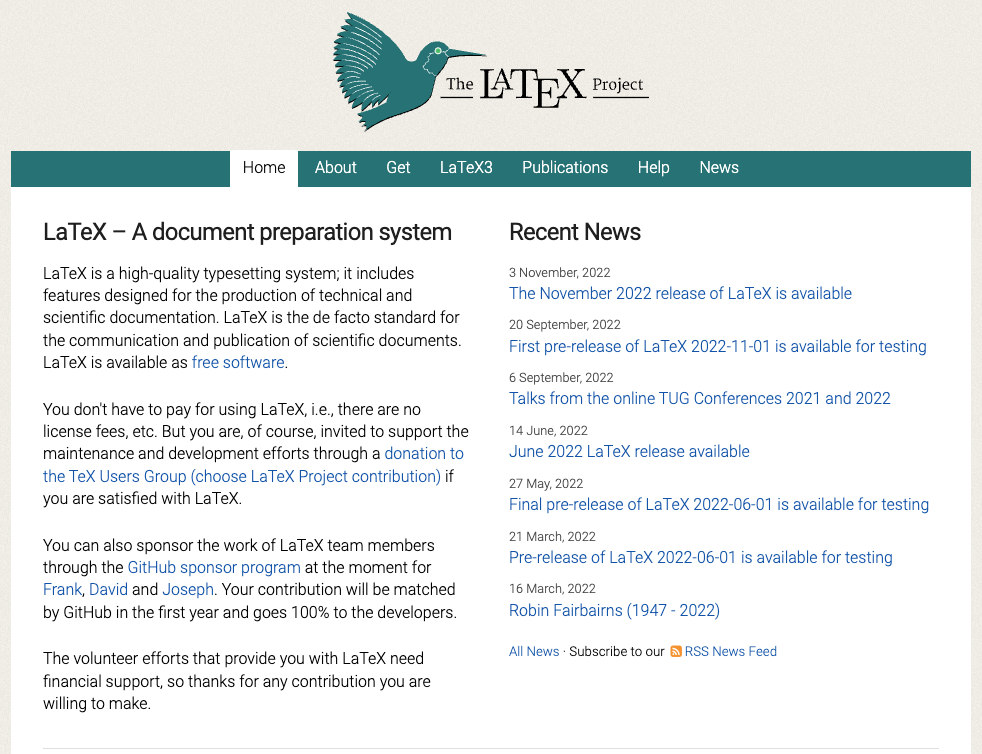
\includegraphics[width=0.7\textwidth]{figures/fig_latex_project}
\par\end{centering}

\caption{LaTeX Project}
\end{figure}


Puede obtener, en forma gratuita, las distribuciones de \LaTeX{},
según su plataforma, en:

\begin{description}
\item [Windows] \href{http://miktex.org/}{http://miktex.org/}; también puede
ocupar \href{http://www.tug.org/protext/}{http://www.tug.org/protext/}.

MikTex ofrece una versión básica. Después de instalarlo, asegúrese de descargar los paquetes adicionales requeridos para compilar esta plantilla.

\item [MacOS] \href{http://www.tug.org/mactex/}{http://www.tug.org/mactex/}.

La versión de MacTex es completa e incluye por defecto todos los paquetes necesarios para compilar esta plantilla.

\item [Unix/Linux] \href{http://www.tug.org/texlive/}{http://www.tug.org/texlive/}.

La instalación de TexLive en plataformas *nix es muy sencilla y directa a través de una consola (con permisos de administración):

(K/X)Ubuntu / Debian: \inlinecode{# apt-get install texlive}

Fedora: \inlinecode{# dnf install texlive}

RedHat / CentOS: \inlinecode{# yum install texlive}
\end{description}

Para una referencia completa sobre \LaTeX{}, recomendamos el libro
de \parencite{Lamport94}; aunque para solucionar problemas específicos,
su mejor aliado es Internet. Otros libros que puede consultar se presentan
en la Bibliografía \parencites{Mittelbach04}{Oetiker06}{Roberts05}{Borbon2014}. %Mittelbach04,Oetiker06,Roberts05,Borbon2014}.


\section{Editores para \LaTeX}
Existen muchos editores de \LaTeX, la mayoría de ellos de distribución gratuita y con versiones para los distintos sistemas operativos:
\begin{description}
    \item [TexStudio] Mac, Windows y Linux. \href{www.texstudio.org}{www.texstudio.org}.
    \item [TexMaker] Mac, Windows y Linux.  \href{https://www.xm1math.net/texmaker/}{https://www.xm1math.net/texmaker/}.
    \item[TeXworks] Mac, Window y Linux. \href{https://www.tug.org/texworks/}{https://www.tug.org/texworks/}
    \item [TexShop] Mac. \href{http://pages.uoregon.edu/koch/texshop/}{http://pages.uoregon.edu/koch/texshop/}.
    \item[Gnome Latex] Linux. \href{https://gitlab.gnome.org/swilmet/gnome-latex}{https://gitlab.gnome.org/swilmet/gnome-latex}.
    \item [Vim + Latex Suite] Mac, Windows y Linux. \href{https://www.vim.org}{https://www.vim.org}.
    \item [LyX] Mac, Windows y Linux. \href{https://www.lyx.org}{https://www.lyx.org}.
    \item [Overleaf] Online. \href{https://www.overleaf.com}{https://www.overleaf.com}.
    \item [Papeeria] Online. \href{https://papeeria.com/landing}{https://papeeria.com/landing}.
    \item [Authorea] Online. \href{https://www.authorea.com}{https://www.authorea.com}.
    \item [\LaTeX{} Base] Online. \href{https://latexbase.com/}{https://latexbase.com/}.
    \item [Latex Workshop for VCode] VCode Plugin. \href{https://marketplace.visualstudio.com/items?itemName=James-Yu.latex-workshop}{https://marketplace.visualstudio.com/}.
\end{description}

%%!TEX root = ../memoria.tex

\chapter{TikZ y PGF (Opciones Avanzadas de Gráficos)}

Los packetes Ti\emph{k}Z y PGF ofrecen alternativas para la creación de gráficos con las más diversas formas y opciones. Para ver opciones consultar \href{http://www.texample.net/tikz/}{www.texample.net/tikz/}.


\newcommand{\MonetaryLevel}{Monetary level}
\newcommand{\RealLevel}{Real level}
\newcommand{\Firms}{Firms}
\newcommand{\Households}{Households}
\newcommand{\Banks}{Banks}
\newcommand{\Commodities}{Commodities}
\newcommand{\LaborPower}{Labor power}
\newcommand{\Wages}{Wages}
\newcommand{\Consumption}{Consumption}
\newcommand{\Credits}{Credits}
\newcommand{\Withdrawals}{Withdrawals}
\newcommand{\Deposits}{Deposits}
\newcommand{\Repayments}{Repayments}

\newcommand{\yslant}{0.5}
\newcommand{\xslant}{-0.6}

\begin{figure}[ht]
    \centering
    \newcounter{density}
    \setcounter{density}{20}
    \begin{tikzpicture}
      \def\amarillo{yellow}
      \def\rojo{red}
      \path[coordinate] (0,0)  coordinate(A)
        ++( 60:5cm) coordinate(B)
        ++(-60:5cm) coordinate(C);
      \path[coordinate] (0,0)  coordinate(D)
        ++(60:5cm) coordinate(E)
        ++(180:5cm) coordinate(F);
      \draw[fill=\amarillo!\thedensity] (A) -- (B) -- (C) -- cycle;
      \draw[fill=\rojo!\thedensity] (D) -- (E) -- (F) -- cycle;
      \foreach \x in {1,...,15}{%
        \pgfmathsetcounter{density}{\thedensity+10}
        \setcounter{density}{\thedensity}
        \path[coordinate] coordinate(X) at (A){};
        \path[coordinate] (A) -- (B) coordinate[pos=.15](A)
          -- (C) coordinate[pos=.15](B)
          -- (X) coordinate[pos=.15](C);
        \draw[fill=\amarillo!\thedensity] (A)--(B)--(C)--cycle;
      }
      \setcounter{density}{20}
      \foreach \x in {1,...,15}{%
        \pgfmathsetcounter{density}{\thedensity+10}
        \setcounter{density}{\thedensity}
        \path[coordinate] coordinate(X) at (D){};
        \path[coordinate] (D) -- (E) coordinate[pos=.15](D)
          -- (F) coordinate[pos=.15](E)
          -- (X) coordinate[pos=.15](F);
        \draw[fill=\rojo!\thedensity] (D)--(E)--(F)--cycle;
      }
    \end{tikzpicture}
    \caption[Gráficos Avanzados con Tikz]{Gráficos Avanzados con Tikz\\ {\scriptsize (Fuente: \url{www.texample.net})}}
    \label{fig:tikz-rt}
\end{figure}



\begin{figure}[ht!]
\centering
% Styles
\tikzstyle{load}   = [ultra thick,-latex]
\tikzstyle{stress} = [-latex]
\tikzstyle{dim}    = [latex-latex]
\tikzstyle{axis}   = [-latex,black!55]

% Drawing Views
\tikzstyle{isometric}=[x={(0.710cm,-0.410cm)},y={(0cm,0.820cm)},z={(-0.710cm,-0.410cm)}]
\tikzstyle{dimetric} =[x={(0.935cm,-0.118cm)},y={(0cm,0.943cm)},z={(-0.354cm,-0.312cm)}]
\tikzstyle{dimetric2}=[x={(0.935cm,-0.118cm)},z={(0cm,0.943cm)},y={(+0.354cm,+0.312cm)}]
\tikzstyle{trimetric}=[x={(0.926cm,-0.207cm)},y={(0cm,0.837cm)},z={(-0.378cm,-0.507cm)}]

  \begin{tikzpicture}[scale=.8]
    \node (origin) at (0,0) {}; % shift relative baseline
    \coordinate (O) at (2,3);
    \draw[fill=gray!10] (O) circle (1);
    \draw[fill=white] (O) circle (0.75) node[below,yshift=-1.125cm] {Signpost Cross Section};
    \draw[dim] (O) ++(-0.75,0) -- ++(1.5,0) node[midway,above] {$d_i$};
    \draw[dim] (O) ++(-1,1.25) -- ++(2,0) node[midway,above] {$d_o$}; 
    \foreach \x in {-1,1} {
      \draw (O) ++(\x,0.25) -- ++(0,1.25);
    }
  \end{tikzpicture}%
  \begin{tikzpicture}[dimetric2]
        \coordinate (O) at (0,0,0);
        \draw[axis] (O) -- ++(6,0,0) node[right] {$x$};
        \draw[axis] (O) -- ++(0,6,0) node[above right] {$y$};
        \draw[axis] (O) -- ++(0,0,6) node[above] {$z$};
        \draw[fill=gray!50] (0,0,-0.5) circle (0.5); 
        \fill[fill=gray!50] (-0.46,-0.2,-0.5) -- (0.46,0.2,-0.5) -- (0.46,0.2,0) -- (-0.46,-0.2,0) -- cycle;
        \draw[fill=gray!20] (O) circle (0.5);
    \draw (0.46,0.2,-0.5) -- ++(0,0,0.5) node[below right,pos=0.0] {Fixed Support};
    \draw (-0.46,-0.2,-0.5) -- ++(0,0,0.5);
    \draw[fill=gray!10] (O) circle (0.2);
    \fill[fill=gray!10] (-0.175,-0.1,0) -- (0.175,0.1,0) -- ++(0,0,4) -- (-0.175,-0.1,4) -- cycle;
    \draw (-0.175,-0.1,0) -- ++(0,0,4);
    \draw (0.175,0.1,0) -- ++(0,0,4) node[right,midway] {Steel Post};
    \draw (4,0,3.95) -- ++(0,0,-1);
    \foreach \z in {0.5,0.75,...,5} {
      \draw[-latex] (-2*\z/5-0.2,0,\z) -- (-0.2,0,\z);
    }
    \draw[load] (0,0,4) -- ++(0,0,-1.25) node[right,xshift=0.1cm] {$F_{z1}$};
    \draw[fill=gray!20] (-0.25,-0.25,5) -- (4,-0.25,5) -- (4,+0.25,5) -- (-0.25,+0.25,5) -- cycle; 
    \draw[fill=gray!50] (+4.00,-0.25,4) -- (4,+0.25,4) -- (4,+0.25,5) -- (+4.00,-0.25,5) -- cycle; 
    \draw[fill=gray!10] (-0.25,-0.25,4) -- (4,-0.25,4) -- (4,-0.25,5) -- (-0.25,-0.25,5) -- cycle; 
    \draw (4.05,0,4) -- ++(1,0,0);
    \draw (4.05,0,5) -- ++(1,0,0);
    \draw[dim] (4.5,0,0) -- ++(0,0,4) node[midway,right] {$h_1$};
    \draw[dim] (4.5,0,4) -- ++(0,0,1) node[midway,right] {$h_2$};
    \draw[dim] (0,0,3.4) -- ++(4,0,0) node[midway,below] {$b_2$};
    \coordinate (P) at (2,-0.25,4.5);
    \draw (P) -- ++(0,0,0.25);
    \draw (P) -- ++(0.25,0,0);
    \draw[dim] (2.125,-0.25,4.5) -- ++(0,0,-0.5) node[midway,right] {$z_1$};
    \draw[dim] (2,-0.25,4.625) -- ++(-2,0,0) node[midway,below] {$x_1$};
    \draw[load] (2,-2.45,4.5) -- ++(0,2.2,0) node[pos=0.0,right,xshift=0.08cm] {$F_{y1}$};
    \draw[axis,dashed,-] (O) -- (0,0,5);
    \draw (0,0,5.5) -- ++(4,0,0) node[midway,above] {$w_{z}$};
    \foreach \x in {0,0.25,...,4} {
      \draw[-latex] (\x,0,5.5) -- ++(0,0,-0.5);
    }
    \draw (-0.2,0,0) -- ++(-2,0,5) node[above,xshift=0.5cm] {$w_{x}=\frac{z}{h_1+h_2} w_0$};
  \end{tikzpicture} 
  \caption [Cargas aplicadas sobre un poste.]{Cargas aplicadas sobre un poste.\\ {\scriptsize (Fuente: \url{www.texample.net})}}
\end{figure}




\begin{figure}[ht]
    \centering
    \begin{tikzpicture}[scale=1,every node/.style={minimum size=1cm},on grid]

	% Real level
	\begin{scope}[
		yshift=-120,
		every node/.append style={yslant=\yslant,xslant=\xslant},
		yslant=\yslant,xslant=\xslant
	] 
		% The frame:
		\draw[black, dashed, thin] (0,0) rectangle (7,7); 
		% Agents:
		\draw[fill=red]  
			(5,2) circle (.1) % Firms
			(2,2) circle (.1); % Households
		% Flows:
		\draw[-latex,thin] 
			(2,1.8) to[out=-90,in=-90] (5,1.8); % Labour Powers
		\draw[-latex,thin]
			(5,2.2) to[out=90,in=90] (2,2.2); % Wages
		 % Labels:
		\fill[black]
			(0.5,6.5) node[right, scale=.7] {\RealLevel}	
			(5.1,1.9) node[right,scale=.7]{\textbf{\Firms}}
			(1.9,1.9) node[left,scale=.7]{\textbf{\Households}}
			(2.2,3) node [scale=.6, rotate=40] {\Commodities} 
			(4.8,1) node [scale=.6, rotate=40] {\LaborPower};	
	\end{scope}
	
	% 2 vertical lines for linking agents on the 2 levels
	\draw[ultra thin](3.8,4) to (3.8,-0.32);
	\draw[ultra thin](.8,2.4) to (.8,-1.8);
	
	% Monetary level
	\begin{scope}[
		yshift=0,
		every node/.append style={yslant=\yslant,xslant=\xslant},
		yslant=\yslant,xslant=\xslant
	]
		% The frame:
		\fill[white,fill opacity=.75] (0,0) rectangle (7,7); % Opacity
		\draw[black, dashed, thin] (0,0) rectangle (7,7); 
		 % Agents:
		\draw [fill=red]
			(5,2) circle (.1) % Firms
			(2,2) circle (.1) % Households
			(3.5,5) circle (.1); % Banks
		 % Monetary Flows:
		\draw[-latex, thin]
			(3.65,5.1) to[out=30,in=30] (5.15,2.1); % Credits
		\draw[-latex, thin]
			(5,1.8) to[out=-90,in=-90] (2,1.8); % Wages
		\draw[-latex, thin]
			(1.9,2.1) to[out=150,in=150] (3.4,5.1);  % Deposits
		\draw[-latex, thin]
			(3.6,4.9) to[out=-30,in=-30] (2.1,1.9); % Withdrawals
		\draw[-latex, thin]
			(2,2.2) to[out=90,in=90] (5,2.2); % Consumption
		\draw[-latex, thin]
			(4.85,1.9) to[out=210,in=210] (3.35,4.9) ; % Repayments
		 % Labels:
		\fill[black]
			(0.5,6.5) node[right, scale=.7] {\MonetaryLevel}
			(5.1,1.9) node[right,scale=.7]{\textbf {\Firms}}
			(1.9,1.9) node[left,scale=.7]{\textbf {\Households}}
			(3.5,5.1) node[above,scale=.7]{\textbf {\Banks}}
			(5.5,2.8) node [above, scale=.6, rotate=-100] {\Credits}
			(2.6,1.3) node [above, scale=.6, rotate=-10] {\Withdrawals}
			(2.9,4.25) node [above, scale=.6, rotate=50] {\Repayments}
			(2.6,5) node [above, scale=.6, rotate=25] {\Deposits}
			(4.7,2.9) node [above, scale=.6, rotate=-60] {\Consumption}
			(2.3,1.3) node [below, scale=.6, rotate=-40] {\Wages}; 
	\end{scope} 
    \end{tikzpicture}
    \caption[Gráficos Avanzados con Tikz]{Gráficos Avanzados con Tikz\\ {\scriptsize (Fuente: \url{www.texample.net})}}
    \label{fig:tikz}
\end{figure}





%---------------------------------------------------------------------------
%%%%%%%%%%%%%%%%%%%%%%%%%%%%%%%%%%%%%
%	Bibliografía
%%%%%%%%%%%%%%%%%%%%%%%%%%%%%%%%%%%%%
\begin{spacing}{1}      % Single space for Bibliography
    \printbibliography
\end{spacing}


%---------------------------------------------------------------------------
%%%%%%%%%%%%%%%%%%%%%%%%%%%%%%%%%%%%%
%	Anexos (Opcional)
%%%%%%%%%%%%%%%%%%%%%%%%%%%%%%%%%%%%%
\begin{appendix}
    %%!TEX root = memoria.tex
\chapter{LICENCIA}\label{appx:licencia}

{\footnotesize
\verbatiminput{LICENSE} 
}

\chapter{Código fuente de figuras y tablas}
\label{annex:code}

\section{Tablas}

\subsection{Tabla Normal}

\begin{Verbatim}[frame=lines, label=\autoref{tbl:temperaturas} Ejemplo Tabla
				, fontsize=\footnotesize, numbers=left
				, baselinestretch=1
				, formatcom=\color{gray}]
\begin{table}[ht]
    \caption[Ejemplo: Tabla de Temperaturas]{Tabla de Temperaturas}
    \label{tbl:annex-table}
    \begin{tabularx}{\linewidth}{@{} l  c  c  X @{}}
        \toprule
        \textbf{\textsc{Day}} &  \textbf{\textsc{Min Temp}} 
        		& \textbf{\textsc{Max Temp}} & \textbf{\textsc{Summary}}\\
    	  \hline\hline
        Monday & 11C & 22C & A clear day with lots of sunshine.
        However, the strong breeze will bring down the temperatures. \\ \hline
        Tuesday & 9C & 19C & Cloudy with rain, across many northern regions. Clear spells
        across most of Scotland and Northern Ireland,
        but rain reaching the far northwest. \\ \hline
        Wednesday & 10C & 21C & Rain will still linger for the morning.
        Conditions will improve by early afternoon and continue
        throughout the evening. \\
        \bottomrule
    \end{tabularx}
\end{table}
\end{Verbatim}

\subsection{Tabla Rotada}

\begin{Verbatim}[frame=lines, label=\autoref{tbl:example-sidewaystable} Ejemplo Tabla Rotada
, fontsize=\footnotesize, numbers=left
, baselinestretch=1
, formatcom=\color{gray}]
\begin{sidewaystable}
    \centering
    \caption[Ejemplo: Rotación de Tablas]{Rotación de Tablas}
    \label{tbl:annex-table-rotated}
    \begin{tabularx}{\columnwidth}{@{}XX@{}}
        \toprule
        \textbf{Column 1} & \textbf{Column 2}\\
        \hline
        \hline
        Second First & Second Second\\
        \blindtext & \blindtext\\
        \bottomrule
    \end{tabularx}
\end{sidewaystable}
\end{Verbatim}


\subsection{Imágenes}

\begin{Verbatim}[frame=lines, label=Incorporar \autoref{fig:logoind}
				, fontsize=\footnotesize, numbers=left
				, baselinestretch=1
				, formatcom=\color{gray}]
\begin{figure}[ht!]
\centering

\includegraphics[width=.3\textwidth]{figures/logoind.png}
\caption[Logotipo Departamento de Industrias]{Logotipo Departamento de Industrias\\
{\scriptsize (Fuente: Departamento de Industrias)}}
\label{fig:annex-logoind}
\end{figure}
\end{Verbatim}

\subsection{Imágenes Flotantes}
\begin{Verbatim}[frame=lines, label=\autoref{fig:emblem-float}
				, fontsize=\footnotesize, numbers=left
				, baselinestretch=1
				, formatcom=\color{gray}]
\begin{wrapfigure}{o}{.4\textwidth}
    \vspace{-20pt}
    \begin{spacing}{1}
        \begin{center}
            
\includegraphics[width=.35\columnwidth]{figures/escudo-utfsm.png}
            \vspace{-10pt}
            \caption{Escudo UTFSM (Flotante)}
            \label{fig:annex-emblem-float}
        \end{center}
    \end{spacing}
    \vspace{-10pt}
\end{wrapfigure}
\end{Verbatim}


    %%!TEX root = ../memoria.tex

\chapter{Otros Formatos UTFSM para Memorias y Tesis de Grado [Obsoleto]}

\section{Otros Formatos UTFSM [OBSOLETO]}

Todo archivo para titulación actualmente se maneja exclusivamente en formato digital.

Las siguientes secciones se mantienen sólo para fines de legado y registro histórico.

\subsection{Formato de las Cubiertas (Empaste)}

A partir del año 2016, ya no es necesaria la entrega de una copia física de la memoria o tesis, siendo esto opcional. Si decide imprimirla, estás son las normas para el empaste.

La cubierta o tapa será de empaste duro, cubierta de vinilo o similar de color NEGRO con letras doradas, según se muestran en \autoref{fig:thesis_cover} y \autoref{fig:thesis_cover_lateral}.

\begin{figure}[ht!]
\centering

\includegraphics[width=.7\textwidth]{figures/thesis_cover.png}
\caption{Cubierta (Empaste) Memorias y Tesis UTFSM.}
\label{fig:thesis_cover}
\end{figure}

\begin{figure}[ht!]
\centering

\includegraphics[width=.7\textwidth]{figures/thesis_cover_lateral.png}
\caption{Lomo del Empaste para Memorias y Tesis UTFSM.}
\label{fig:thesis_cover_lateral}
\end{figure}

\subsection{Formato del Disco Compacto}

El CD/DVD debe tener una carátula de identificación circular con fondo blanco, conteniendo las siguientes leyendas:

\begin{itemize}
		\item
    Centrado en la parte superior: UTFSM, con letras mayúsculas en negrita tamaño 12. A renglón seguido el nombre de la Unidad Académica con letras mayúsculas en negrita tamaño 10.
		\item
    Centrado en la parte inferior el nombre completo del alumno con letras mayúsculas en negrita tamaño 10.
		\item
    Tres espacios más abajo y centrado, “TÍTULO DE LA MEMORIA”, con letras mayúsculas en negrita tamaño 10.
		\item
    Dos espacios más abajo y centrado MES –AÑO, con letras mayúsculas en negrita tamaño 10.
    En el lado izquierdo y centrado, el escudo en colores de la Institución.
		\item
    En el lado derecho y centrado, NOMBRE DE LA UNIDAD ACADÉMICA y la ubicación CIUDAD – PAIS, con letras mayúsculas en negrita tamaño 8.
\end{itemize}

\begin{figure}[ht!]
\centering
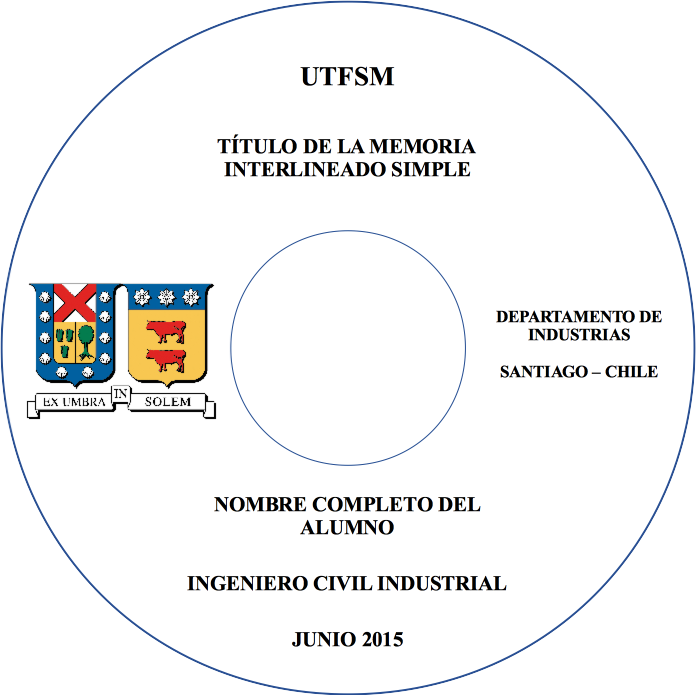
\includegraphics[width=.4\textwidth]{figures/thesis_cd.png}
\caption{Disco Compacto para Memoria UTFSM}
\label{fig:thesis_cd}
\end{figure}


Los CD se guardarán, en la biblioteca, en una caja de acrílico que tendrá una carátula de identificación dividida en tres franjas iguales, con las siguientes leyendas:
\begin{itemize}
		\item
    El escudo a color de la Institución de 20 mm de alto, centrado en la franja superior.
		\item
    El nombre completo del alumno, y centrado dos espacios más abajo el título de la memoria, en la franja del medio
		\item
    El nombre de la Unidad Académica, y renglón más abajo, año. En la franja inferior.
\end{itemize}


\begin{figure}[ht!]
    \centering
    
\includegraphics[width=.4\textwidth]{figures/thesis_cd_cover.png}
    \caption{Cubierta de Disco Compacto para Memorias y Tesis UTFSM.}
    \label{fig:thesis_cd_cover}
\end{figure}



    %...                  % Agregar más apéndices
\end{appendix}

\end{document}
